\documentclass[a4paper,fleqn]{cas-sc}   %{article}
%remove ORCID footnote
\renewcommand{\printorcid}{}


%\usepackage{natbib}
% cas-common.sty references \bibsep (a natbib length) even when natbib is not loaded.
% Declaring it here prevents the "Undefined control sequence" error at \begin{document}.
\newlength{\bibsep}
\usepackage{float}
\usepackage{pdflscape}
\usepackage{array}
\usepackage{multirow}
\usepackage{booktabs}
\usepackage{longtable}
\usepackage{caption}
\captionsetup[longtable]{labelfont=bf,labelsep=newline,singlelinecheck=false,justification=raggedright}
\usepackage{adjustbox}
\usepackage[style=authoryear-icomp,
uniquelist=false,
maxnames=2,
minnames=1,
maxbibnames=99,
    backend=biber, giveninits=true,
    ibidtracker=false,
    uniquename=false,
    natbib=true]{biblatex}

\addbibresource{DCE_lit_review.bib}
\addbibresource{used_EV_lit_review.bib}
\addbibresource{Used EV.bib}
\addbibresource{EV battery.bib}
% \DeclareNameAlias{default}{family-given}

\usepackage{amsmath}
\usepackage{amssymb}
\usepackage{bm}
\usepackage{hyperref}
\usepackage{graphicx}

% Force floats to appear where inserted, not deferred to end of document.
% Use [H] specifier on every \begin{figure} and \begin{table}.
% The parameters below allow LaTeX to place floats very liberally.
\renewcommand{\topfraction}{0.99}
\renewcommand{\bottomfraction}{0.99}
\renewcommand{\textfraction}{0.01}
\renewcommand{\floatpagefraction}{0.99}
\setcounter{topnumber}{20}
\setcounter{bottomnumber}{20}
\setcounter{totalnumber}{40}

% TRD: double-spaced text, no manuscript line numbers (added by the submission system)
\usepackage{setspace}

%\usepackage{titlesec}
%\titlespacing*{\section}{0pt}{6pt}{3pt}  
%\titlespacing*{\subsection}{0pt}{6pt}{3pt} 
%\titlespacing*{\subsubsection}{0pt}{6pt}{3pt}

% remove the "preprint"
\ExplSyntaxOn \cs_gset:Npn \__first_footerline: { \group_begin: \small \sffamily \__short_authors: \group_end: } \ExplSyntaxOff

\shortauthors{}

%%%Author macros
\def\tsc#1{\csdef{#1}{\textsc{\lowercase{#1}}\xspace}}
\tsc{WGM}
\tsc{QE}
\tsc{EP}
\tsc{PMS}
\tsc{BEC}
\tsc{DE}
%%%


\begin{document}
\let\WriteBookmarks\relax
\def\floatpagepagefraction{1}
\def\textpagefraction{.001}
\shorttitle{}
%\shortauthors{X. Iogansen et~al.}

%\begin{frontmatter}

\title [mode = title]{Consumer Valuation of Used vehicle attributes}


\author[1]{Zain {Hoda}}
\fnmark[1]
\credit{Conceptualization, Data curation, Methodology, Software, Formal analysis, Writing -- original draft, Writing -- review \& editing}

\author[1,2]{Xiatian {Iogansen}}
\fnmark[2]
\credit{Conceptualization, Data curation, Methodology, Writing -- review \& editing}

\author[2]{Christina {Gore}}
\credit{Conceptualization, Data curation, Methodology, Investigation, Writing -- original draft, Writing -- review \& editing, Supervision, Project administration, Funding acquisition}
\fnmark[3]
\cormark[1]
\cortext[cor1]{Corresponding author. Email: jph@gwu.edu}

\author[2]{Joshua D. {Kneifel}}
\credit{Conceptualization, Data curation, Methodology, Investigation, Writing -- review \& editing, Supervision, Project administration, Funding acquisition}
\fnmark[4]

\author[1,2]{Sindhu {Ranganath}}
\credit{Data curation, Writing -- original draft, Writing -- review \& editing}
\fnmark[5]

\author[1]{John {Helveston}}
\credit{Conceptualization, Methodology, Writing -- review \& editing, Supervision}
\fnmark[6]


                
\affiliation[1]{organization={Department of Engineering Management and Systems Engineering, George Washington University},
                addressline={800 22nd Street NW},
                city={Washington},
                state={DC},
                postcode={20052},
                country={USA}}

\affiliation[2]{organization={Applied Economics Office, Engineering Laboratory, National Institute of Standards and Technology},
                addressline={100 Bureau Drive},
                city={Gaithersburg},
                state={MD},
                postcode={20899},
                country={USA}}
                


\fntext[fn1]{zain.hoda@gwu.edu, https://orcid.org/0009-0003-0958-1868}
\fntext[fn2]{xiatian.iogansen@gwu.edu \& xiatian.iogansen@nist.gov, https://orcid.org/0000-0002-4851-1323}
\fntext[fn3]{christina.gore@nist.gov, https://orcid.org/0000-0002-3586-6918}
\fntext[fn4]{joshua.kneifel@nist.gov}
\fntext[fn5]{sindhu.ranganath@nist.gov, https://orcid.org/0000-0001-5764-9773}
\fntext[fn6]{jph@gwu.edu, https://orcid.org/0000-0002-2657-9191}


\begin{abstract}
We estimate willingness to pay (WTP) for powertrain and vehicle attributes in the U.S. used-vehicle market using a discrete choice experiment with 2,254 adults planning to buy a used car or SUV within two years, and compare the estimates with observed prices. Choice tasks varied powertrain (conventional, hybrid, battery electric), price, operating cost, range, vehicle age, and mileage. Four mixed logit models were estimated by vehicle segment and budget tier. The battery electric vehicle (BEV) powertrain carries a significant WTP penalty relative to conventional vehicles in every model, with large standard deviations indicating heterogeneous rather than uniformly averse preferences. Driving range narrows the BEV penalty, which is indistinguishable from zero only for high-budget car buyers. Matched real-market pairs show mixed results: two low-budget BEVs are priced well above WTP-implied values, a high-budget car BEV is consistent with it, and hybrid premiums fall below or above it.
\end{abstract}

\begin{highlights}
\item Segment and budget tier shape the used-BEV valuation gap.
\item BEVs carry a WTP penalty in every segment that narrows with driving range
\item Hybrids earn a WTP premium only among high-budget buyers
\item WTP-implied values are compared with prices of matched real used vehicles
\item Low-budget BEVs are priced well above WTP; high-budget cars are near parity
\end{highlights}



\begin{keywords}
Battery electric vehicle \sep Used vehicle market \sep Discrete choice experiment \sep Willingness to pay \sep Mixed logit \sep Consumer preferences
\end{keywords}

\maketitle
\doublespacing
\section{Introduction}
\label{section:intro}
The transition of light-duty vehicles to electric powertrains is a central concern of transport and environmental policy, and its pace depends not only on new-vehicle sales but also on the secondary market through which most vehicles change hands. Used vehicles account for approximately 70\% of vehicle transactions in the United States \parencite{bts2023}. Used-vehicle buyers typically face tighter budgets and greater uncertainty about vehicle condition than new-vehicle buyers \parencite{trd2024usedEV_adoption, robersonNotAllSubsidies2022, fernandesUSUnderstandingConsumer2023}, yet stated-preference evidence on how they value electric powertrains remains limited.

Used battery electric vehicles (BEVs) matter to the transition beyond their transaction volume. They offer a lower-cost entry point to electric mobility for households that cannot afford a new vehicle \parencite{canepaEarlyLookPlugin2019, hagmanTotalCostOwnership2016, sheykhfardAnalyzingPurchaseIntentions2025}, and so could extend the emissions benefits of electrification beyond early adopters \parencite{sheykhfardAnalyzingPurchaseIntentions2025, trd2024usedEV_concerns, tandf2025usedEV}. Their expected resale value shapes the economics of new-BEV adoption, and concern about it (resale anxiety) is a recognized barrier \parencite{bruckmannResaleAnxietyObstacle2021, limMassAdoptionElectric2015}. Extending the life of vehicles and battery packs may also reduce demand for battery materials and support a circular economy \parencite{guzekElectricVehiclesOverview2024, husterConsumersWantReconditioned2024, shaikhSystemDynamicsCosting2023}.

Used BEVs share the range anxiety, charging-access concerns, and upfront cost premium of EVs \parencite{sheykhfardAnalyzingPurchaseIntentions2025}, and buyers additionally cannot directly observe the condition of a used BEV. Uncertainty about prior condition and reliability is reported to be a primary purchase deterrent \parencite{fernandesUSUnderstandingConsumer2023}. Because battery aging depends on operating temperature, charging behavior, and depth of discharge as well as time \parencite{guzekElectricVehiclesOverview2024}, it is not captured by age or odometer readings alone, so these two attributes may carry more of the discount for a used BEV than for a conventional vehicle.

Research on EV consumer preferences has concentrated predominantly on new-vehicle buyers \parencite{sheykhfardAnalyzingPurchaseIntentions2025, tandf2025usedEV}. The smaller body of work on used EVs draws largely on current owners or convenience samples \parencite{trd2024usedEV_concerns, sheykhfardAnalyzingPurchaseIntentions2025}, which may not represent prospective buyers (Section~\ref{section:lit_review}). As a result, there is limited stated-preference evidence on prospective used-BEV buyers that takes their budgets into account. Budget is central in this market: it determines which vehicles fall within a buyer's realistic consideration set and how sensitive the buyer is to price, and lower-budget buyers face fewer BEV options and higher relative cost burdens \parencite{konstantinou2024usedEV_price, trd2024usedEV_concerns}. Estimates that pool buyers across budgets may therefore misstate how much the BEV valuation gap depends on who is buying, and how much it would take to close it.

This study reports willingness-to-pay (WTP) estimates for powertrain type, driving range, vehicle age, mileage, and operating cost from a discrete choice experiment (DCE) with prospective used-vehicle buyers in the United States, described in Section~\ref{section:survey}. Estimates are stratified along two dimensions, vehicle type and budget. Vehicle type (car or SUV) is included because buyers in the two segments may value attributes differently, and prior work analyzes them separately \parencite{forsytheDrivingElectricVehicle}. Budget tier (low or high) is included for the reasons mentioned in the previous paragraph.

This study makes three contributions. First, it provides WTP estimates for powertrain type, driving range, vehicle age, mileage, and operating cost from prospective used-vehicle buyers, estimated separately for cars and SUVs within low- and high-budget tiers. Second, it quantifies the BEV valuation gap relative to a conventional vehicle in each budget tier and vehicle segment, and how much of that gap driving range closes within and beyond the ranges respondents evaluated. Third, it compares WTP-implied values with the observed prices of matched real-market vehicle pairs, illustrating where stated preferences and used-market pricing align and diverge.

The study addresses two research questions:
\begin{enumerate}
\item What is willingness to pay for used-vehicle attributes (powertrain type, driving range, vehicle age, mileage, and operating cost) in each vehicle segment and budget tier?
\item How do observed used-market price premiums for BEVs and HEVs, relative to matched conventional counterparts at approximately three years of age, compare with the premiums implied by estimated WTP?
\end{enumerate}

The remainder of the paper is organized as follows. Section~\ref{section:lit_review} reviews the literature on used-vehicle markets, general EV adoption determinants, and consumer preferences for used EVs. Section~\ref{section:survey} describes the survey design, data collection, and sample profile, and Section~\ref{section:method} presents the mixed logit specification and estimation. Section~\ref{section:results} reports the mixed logit estimates. Section~\ref{section:analysis} converts them to willingness to pay for each attribute and segment, quantifies the BEV valuation gap, and compares WTP-implied values with observed prices of matched used vehicles. Section~\ref{section:discussion} discusses policy implications, and Section~\ref{section:conclusion} concludes. Appendix~\ref{app:gas_sensitivity} tests the sensitivity of the market comparison to gasoline prices.

\section{Literature Review}
\label{section:lit_review}

This review covers four bodies of work: the theoretical and methodological basis for valuing vehicle attributes, the broader used-vehicle market, general determinants of EV adoption, and the emerging literature on used-EV consumer preferences. It closes by identifying the gap this study addresses.

\subsection{Valuing Vehicle Attributes with Discrete Choice Experiments}

Discrete choice experiments (DCEs) are grounded in random utility theory, in which a consumer chooses the alternative with the highest utility and the analyst observes only part of that utility \parencite{trainDiscreteChoiceMethods2009, li2020BEVchoice}. DCEs are widely used to value vehicle attributes because they let researchers vary powertrain, price, range and operating cost independently, including combinations not yet available in the market \parencite{helveston2016EVpreferences, sagepub2020EVattributes}. Mixed logit models extend this framework by allowing preference parameters to vary across individuals, which matters for BEVs, where preference heterogeneity is large and may be bimodal \parencite{helveston2015subsidies}. Estimating the model in willingness-to-pay (WTP) space places the heterogeneity directly on monetary valuations, which makes them easier to interpret and compare across studies \parencite{robersonNotAllSubsidies2022, helveston2015subsidies, trainWeeks2005}. Prior DCEs report WTP for additional driving range and for reduced operating cost \parencite{helveston2015subsidies, forsythe2023technology}. Stated-preference estimates can differ from observed market behavior because of hypothetical bias \parencite{helveston2016EVpreferences, tandf2025usedEV, fifer2014hypothetical}, which is why this study also compares WTP-implied values with observed used-market prices.

\subsection{The Used-Vehicle Market}

Affordability, vehicle condition, and reliability are the dominant purchase criteria for used-vehicle buyers \parencite{consumerreports_usedcar, epa_usedvehicle}, and fuel costs also factor into vehicle choice, particularly among cost-sensitive households. Used-car purchasing is more common among larger households and renters, and low-income single-vehicle renters carry the highest vehicle-cost burdens relative to income \parencite{konstantinou2024usedEV_price}.

These burdens have grown since 2020. Average used-vehicle prices climbed relative to pre-pandemic levels and remained elevated through 2024--2025 \parencite{cox2024usedvehicle_prices}; in April 2025 the average transaction price was \$25,547 \parencite{kbb2025usedcar_price}. Industry surveys report that 74\% of used-vehicle buyers evaluated both new and used options and that 71\% entered the market without a fixed vehicle preference \parencite{cox2025buyerjourney}, and that 43\% of consumers would switch brands to obtain a lower price \parencite{c4analytics2025pricesensitivity}. These figures come from industry sources rather than peer-reviewed studies, but they are consistent with a market in which price pressure widens the set of vehicles buyers consider.

\subsection{General Factors in EV Adoption}

Purchase price, operating costs, driving range, recharging time, charging infrastructure, environmental benefits, and government incentives all shape EV adoption \parencite{sagepub2020EVattributes}. Range and recharging time show statistically significant effects across multiple stated-preference studies \parencite{helveston2016EVpreferences}. Pooled evidence indicates that the range--charging trade-off appears only at higher range: consumers accept shorter range in exchange for denser charging networks only once BEV range exceeds roughly 250--300 km (about 155--185 miles) \parencite{trd2024metaregression}. Below that threshold, additional charging infrastructure does not compensate for range loss. This evidence comes from new-vehicle contexts. Whether it carries over to used BEVs, where battery aging may reduce usable range, has not been tested. Battery warranty and depreciation rate also independently affect purchase intent \parencite{trd2019batterywarranty}.

\subsection{Used Electric Vehicle Adoption}

The U.S. used-EV market passed 400,000 units in 2023, yet studies of consumer preferences in that market remain sparse \parencite{tandf2025usedEV}. Current used-EV owners resemble early adopters of new EVs: they are disproportionately male, middle-aged, highly educated, and higher-income \parencite{trd2024usedEV_concerns, trd2024usedEV_adoption}. Full-time employment and private off-street parking also predict ownership \parencite{trd2024usedEV_adoption}. Because these studies describe current owners, they cannot show whether lower-budget buyers would purchase used BEVs if given the opportunity.

Prospective used-EV buyers cite price, battery performance, and charging access as their principal concerns \parencite{trd2024usedEV_concerns}. Lower-income buyers are more sensitive to both price and charging availability than higher-income buyers \parencite{trd2024usedEV_concerns}, and concern about infrastructure correlates with reluctance to buy \parencite{trd2024usedEV_adoption}. Prior EV ownership works in the opposite direction: experienced EV drivers are more comfortable purchasing pre-owned vehicles, and new EV drivers say they would consider a used EV once range and home-charging needs are met \parencite{trd2024usedEV_adoption}. \textcite{tandf2025usedEV} identify three segments among prospective used-EV buyers: those for whom cost is a binding constraint, those apprehensive about adapting to EV technology, and those drawn by a favorable cost--benefit ratio and lower depreciation risk. Price is a common orientation across segments, but each segment arrives at it through different reasoning, so treating price sensitivity as uniform is not supported by this evidence.

Used-vehicle and new-vehicle buyers show broadly similar EV preference structures, with some differences. Used-vehicle buyers are more sensitive to fast-charging time and to the proximity of slow charging to home, whereas new-vehicle buyers are more sensitive to home-charging availability \parencite{sagepub2020EVattributes, khaloeiHowDoesCharging2020}. The federal incentives available to used-vehicle buyers were also smaller and price-capped \parencite{tandf2025usedEV}.

Average used-EV prices range from \$9,000 to \$37,000 depending on range and vehicle class, against roughly \$14,000 for a comparable used gasoline vehicle \parencite{konstantinou2024usedEV_price}. The size of this gap is relevant to RQ2, which asks how observed price premiums compare with those implied by WTP.

\subsection{Synthesis and Research Gap}

Used-car buyers are more cost-conscious than new-car buyers, and recent price increases have widened that difference. Price drives used-EV interest, but these buyers are not a uniform group: their motivations, incomes, and infrastructure access differ, as does the weight they give to battery performance, range, and charging. Battery warranty and depreciation rate also shape decisions beyond sticker price.

Three limitations in the existing evidence motivate this study. First, several studies on used EVs draw on current owners or convenience samples \parencite{trd2024usedEV_concerns, sheykhfardAnalyzingPurchaseIntentions2025}, which limits what they can say about prospective buyers. Second, although income and budget are repeatedly identified as central to used-EV adoption, stated-preference evidence on how WTP for powertrain, range, and age varies by budget tier is limited. Third, stated-preference estimates are rarely compared with observed used-market prices, so it is unclear whether stated valuations are consistent with what buyers face in the market.

This study addresses these gaps with a DCE of prospective used-vehicle buyers in the United States, stratified by vehicle type and budget tier. It estimates WTP for powertrain type, driving range, vehicle age, mileage, and operating cost, and compares WTP-implied values with the prices of matched real-market vehicles. These gaps motivate the two research questions posed in the Introduction: what WTP for used-vehicle attributes is in each segment and budget tier (RQ1), and how observed used-market price premiums compare with WTP-implied premiums (RQ2).


\section{Survey Design, Data Collection, and Sample Profile}
\label{section:survey}

\subsection{Vehicle Choice Experiment}
\label{subsec:dce_design}

Respondents were screened to U.S. adults who planned to acquire a used car (sedan or hatchback) or SUV (including crossovers) within two years. Respondents were screened out if they planned to buy only new vehicles, were unsure of or planned beyond a two-year purchase window, or intended to buy a van, truck, or other body style. The term ``used'' was deliberately left undefined so that a researcher-supplied definition would not influence respondents' interpretation. Each respondent completed six choice tasks with the same structure: in each task they saw three hypothetical used vehicles and could decline all of them by selecting ``Even if these were my best options, I would not choose any of these vehicles.'' The order of the alternatives within each task was randomized.

To keep the choice tasks realistic, price and attribute levels were calibrated to each respondent's segment. Respondents were routed to one of four designs defined by vehicle type (car or SUV) and stated budget tier (low or high), as shown in Table~\ref{table:dce_attributes}. Budget was elicited before the choice tasks with the question ``What is your budget for the vehicle?'' Car buyers with a stated budget of up to \$20,000 (inclusive) were assigned to the low-budget design and the remainder to the high-budget design; the corresponding cutoff for SUV buyers was \$25,000 (inclusive). The experiment includes six attributes: powertrain, purchase price, model year, mileage, electric range (BEV alternatives only), and operating cost. Three powertrains were included: conventional gasoline vehicles (ICEV), gas hybrid electric vehicles (HEV), and battery electric vehicles (BEV). Age and mileage are primary determinants of used-vehicle value \parencite{prieto2015}, so both are included, with model year serving as the observable proxy for age. Electric range was shown only for BEV alternatives. Attributes that may also influence used-BEV choices, such as brand, charging time, and battery health or warranty, were not varied in this experiment.

Operating-cost levels were derived from observed energy consumption. Consumption (kWh per mile for BEVs, miles per gallon for ICEVs and HEVs) was taken from EPA ratings for 2024 model-year vehicles, by powertrain and body type. These were combined with the 10th--90th percentile range of state-level electricity prices (\$0.11--\$0.33 per kWh) and retail gasoline prices (\$2.66--\$4.77 per gallon) in early 2025 to generate 20 approximately equally spaced values per powertrain--body-type combination. Because fieldwork ran from Dec 2025 to April 2026, some months after the price data, fuel prices during fieldwork may have differed. Costs were shown in cents per mile with the miles-per-gallon equivalent of a gasoline vehicle at the same cost, to allow comparison across powertrains. Ranges were bounded by powertrain: ICEV 9--18 cents per mile for both body types, BEV 3--12 cents per mile for both, and HEV 6--12 cents for cars and 9--18 cents for SUVs. These bounds reflect the plausible fuel-cost range of each powertrain.

Choice sets were generated with the \texttt{cbcTools} R package \parencite{helvestonCbcToolsDesignAnalyze2025}. Profiles were drawn at random from the restricted profile space (with the powertrain-specific operating-cost bounds above), alternatives were balanced across powertrain types, and dominated profiles were excluded. Table~\ref{table:dce_attributes} defines each attribute and lists its levels, and Figure~\ref{fig:vehicle_dce} shows an example choice task.

Price and range levels differ across the four design cells (Table~\ref{table:dce_attributes}). For example, high-budget car buyers saw prices of \$20,000--\$40,000 and low-budget car buyers \$10,000--\$20,000. Differences in estimated WTP between budget tiers therefore combine differences in preferences with differences in the attribute ranges respondents evaluated, and budget is self-reported rather than observed. We return to this in the limitations.

Before the DCE, respondents reported their vehicle budget. To prevent styling from confounding attribute effects, each respondent also chose one image, from nine options within their selected body type, closest to the next vehicle they were considering. That image depicted all alternatives in every choice task, so powertrain, brand, and color were not conveyed visually.

The survey was programmed using the Surveydown package in R and administered online through shinyapps.io. Respondents were recruited from the Dynata and Prolific online panels and both groups were compensated through the panels.

\begin{table}[pos=H]
\caption{BEV choice experiment attributes and levels.}
\label{table:dce_attributes}
\begin{adjustbox}{width=\textwidth, center}
{\renewcommand{\arraystretch}{1.4}
\begin{tabular}{p{3.2cm} p{4.8cm} p{3cm} p{3cm} p{3cm} p{3cm}}
\toprule
\multirow{2}{*}{\textbf{Attribute}} & \multirow{2}{*}{\textbf{Definition}} & \multicolumn{4}{c}{\textbf{Levels}} \\
\cmidrule(lr){3-6}
 & & \textbf{Low-budget Car} \newline ($\leq$\$20,000) & \textbf{High-budget Car} \newline ($>$\$20,000) & \textbf{Low-budget SUV} \newline ($\leq$\$25,000) & \textbf{High-budget SUV} \newline ($>$\$25,000) \\
\midrule
Mileage & The total number of miles a vehicle has traveled since manufacture. & \multicolumn{4}{p{12.5cm}}{\textbf{All levels:} \newline20,000--60,000 miles (5000-mile increments).} \\
\addlinespace[4pt]
Powertrain & The type of powertrain the vehicle runs on. & \multicolumn{4}{p{12.5cm}}{%
  \textbf{All levels:} \newline
  \textit{(1) Conventional:} Gasoline or other liquid-fuel engine, such as diesel or flex-fuel.\newline
  \textit{(2) Gas hybrid electric vehicle (HEV):} Smaller gasoline engine + electric motor + small battery. The gasoline engine recharges the battery to improve fuel efficiency.\newline
  \textit{(3) Battery electric vehicle (BEV):} Electric motor only. Must be plugged into an electrical outlet to be refueled.} \\
\addlinespace[4pt]
Electric Range & Maximum distance the BEVs can travel on a full charge. Applies to BEVs only. & 50--150 miles \newline (50-mile increments) & 100--250 miles \newline (50-mile increments) & 150--250 miles \newline (50-mile increments) & 200--350 miles \newline (50-mile increments) \\
\addlinespace[4pt]
Operating Cost & Cost in cents per mile driven of fueling the vehicle. The equivalent fuel efficiency in miles per gallon (MPG) of a conventional gasoline vehicle is displayed in parenthesis. & \multicolumn{2}{p{6cm}}{%
  \textbf{Car:} \newline
  ICEV: 9--18 cents/mile\newline
  HEV: 6--12 cents/mile\newline
  BEV: 3--12 cents/mile} & \multicolumn{2}{p{6cm}}{%
  \textbf{SUV:} \newline
  ICEV: 9--18 cents/mile\newline
  HEV: 9--18 cents/mile\newline
  BEV: 3--12 cents/mile} \\
\addlinespace[4pt]
Model Year & The actual year the vehicle was made. & \multicolumn{4}{p{12.5cm}}{\textbf{All levels:} \newline 2015--2023 (2-year increments).} \\
\addlinespace[4pt]
Purchase price & The total cost of the vehicle in dollars, including down payment, monthly payments, taxes, and fees. & \$10,000--\$20,000 \newline (\$2,000 increments) & \$20,000--\$40,000 \newline (\$5,000 increments) & \$15,000--\$25,000 \newline (\$5,000 increments) & \$25,000--\$45,000 \newline (\$5,000 increments) \\
\bottomrule
\end{tabular}}
\end{adjustbox}
\end{table}


\begin{figure}[pos=H]
    \centering
    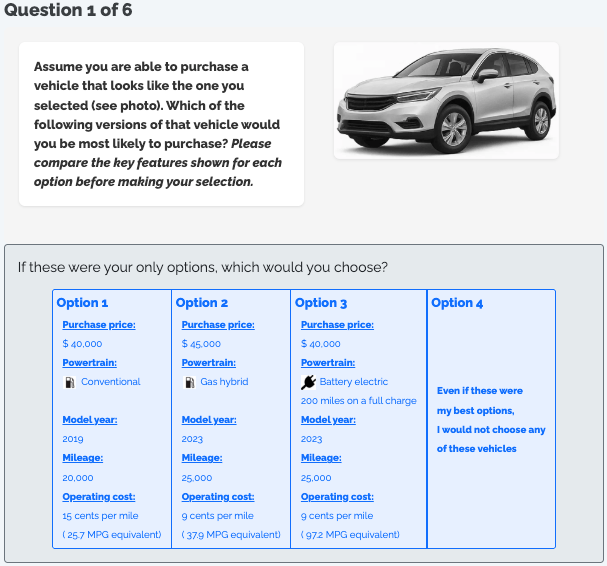
\includegraphics[width=0.7\textwidth]{images/vehicle_analysis/vehicle_choice_image.png}
    \caption{Example of a vehicle choice task presented to respondents. Each task offers three used vehicle alternatives with varying attributes and a ``None of the above'' opt-out option.}
    \label{fig:vehicle_dce}
\end{figure}


\subsection{Data Collection and Sample Profile}
\label{subsec:data}

Online surveys ran in batches on two panels, Dynata and Prolific from December 2025 to April 2026, with a median completion time of approximately 14 minutes.
Of 3,661 respondents who passed the screener (Dynata n = 593; Prolific n = 3,068), 687 failed a comprehension check, in which they were asked to select the dominant alternative in a demonstration choice task, 122 completed the choice section in under 30 seconds, 35 gave the same answer to every choice task, and 464 did not complete all choice tasks. A further 99 Prolific respondents were removed due to mismatch in prolific respondent ids. The final analytic sample is 2,254 respondents (Dynata n = 281; Prolific n = 1,973). The two panels are pooled in the models without a panel indicator (Section~\ref{section:method}).

Compared with ACS 2020--2024 five-year estimates (Table~\ref{table:sample_profile_vehicle}), the sample is younger, more female, better educated, and more renter-heavy, and under-represents households earning \$150,000 or more (13.5\% vs.\ 23.0\%). The ACS describes all U.S. adults, whereas the sample comprises prospective used-vehicle buyers, so some differences need not indicate bias. Even so, the pattern is consistent with online-panel recruitment, and Prolific respondents make up 88\% of the sample. No quotas or weights were applied, so the estimates describe prospective used-vehicle buyers in online panels and should not be read as nationally representative. Gender was self-reported (female, male, or other); the ACS reports a binary classification, so no ACS comparison is available for the ``other'' category.

\begin{table}[pos=H]
\centering
\caption{Sample profile compared with the U.S. population (ACS 2020--2024 5-year estimates).}
\label{table:sample_profile_vehicle}
\begin{tabular}{lrrr}
\toprule
 & Sample (n) & Sample (\%) & ACS (\%) \\
\midrule
\multicolumn{4}{l}{\textit{Age}} \\
\quad 18 - 24 & 329 & 14.7 & 11.7 \\
\quad 25 - 34 & 675 & 30.2 & 17.5 \\
\quad 35 - 44 & 574 & 25.7 & 16.9 \\
\quad 45 - 54 & 344 & 15.4 & 15.6 \\
\quad 55 - 64 & 190 & 8.5 & 16.2 \\
\quad 65+ & 121 & 5.4 & 22.0 \\
\addlinespace[2pt]
\multicolumn{4}{l}{\textit{Gender}} \\
\quad Female & 1,340 & 59.6 & 51.0 \\
\quad Male & 861 & 38.3 & 49.0 \\
\quad Other & 49 & 2.2 & -- \\
\addlinespace[2pt]
\multicolumn{4}{l}{\textit{Race}} \\
\quad White alone & 1,543 & 68.5 & 63.3 \\
\quad Black or African American alone & 322 & 14.3 & 11.9 \\
\quad Other or multiple races & 389 & 17.3 & 24.8 \\
\addlinespace[2pt]
\multicolumn{4}{l}{\textit{Hispanic origin}} \\
\quad Hispanic or Latino & 269 & 11.9 & 17.4 \\
\quad Not Hispanic or Latino & 1,985 & 88.1 & 82.6 \\
\addlinespace[2pt]
\multicolumn{4}{l}{\textit{Household income}} \\
\quad Less than \$25,000 & 343 & 15.2 & 14.6 \\
\quad \$25,000 - \$49,999 & 374 & 16.6 & 16.7 \\
\quad \$50,000 - \$74,999 & 545 & 24.2 & 15.5 \\
\quad \$75,000 - \$99,999 & 257 & 11.4 & 12.6 \\
\quad \$100,000 - \$149,999 & 428 & 19.0 & 17.5 \\
\quad \$150,000 or more & 304 & 13.5 & 23.0 \\
\addlinespace[2pt]
\multicolumn{4}{l}{\textit{Education}} \\
\quad High school or less & 314 & 14.0 & 36.4 \\
\quad Some college or associate & 731 & 32.5 & 27.9 \\
\quad Bachelor's degree & 765 & 34.0 & 21.6 \\
\quad Graduate or professional degree & 438 & 19.5 & 14.1 \\
\addlinespace[2pt]
\multicolumn{4}{l}{\textit{Housing tenure}} \\
\quad Own & 1,087 & 52.0 & 65.2 \\
\quad Rent & 1,002 & 48.0 & 34.8 \\
\addlinespace[2pt]
\multicolumn{4}{l}{\textit{Housing type}} \\
\quad Single-family detached & 1,367 & 60.6 & 62.3 \\
\quad Single-family attached & 227 & 10.1 & 6.4 \\
\quad Apartment (2+ units) & 574 & 25.5 & 26.0 \\
\quad Mobile home or other & 86 & 3.8 & 5.2 \\
\bottomrule
\end{tabular}
\begin{minipage}{0.8\textwidth}
\vspace{4pt}\footnotesize
Notes: Sample size and shares are unweighted and exclude item nonresponse. `--' indicates no comparable ACS category. ACS universes: population 18+ (age, gender, race, Hispanic origin), population 25+ (education), and households (income, tenure, housing type).
\end{minipage}
\end{table}



\subsection{Household Vehicle Context and Used-BEV Purchase Interest}
\label{subsec:household_context}

Table~\ref{table:household_context_vehicle} profiles the households behind the sample. Most own at least one vehicle (35.2\% one, 37.9\% two, 22.9\% three or more; 4.0\% none). A large majority (83.8\%) of those with a primary vehicle drive a conventional gasoline vehicle, with hybrids (10.2\%), battery electric vehicles (4.1\%), and plug-in hybrids (1.8\%) the remainder, so few respondents are current EV owners. Home-charger access is split roughly evenly (44.0\% yes, 49.1\% no). Stated likelihood of buying a used BEV as the next vehicle is concentrated at the unlikely end of the scale (55.1\% somewhat or very unlikely vs.\ 31.3\% somewhat or very likely).

\begin{table}[pos=H]
\centering
\caption{Household vehicle context and used-BEV purchase interest.}
\label{table:household_context_vehicle}
\begin{tabular}{lrr}
\toprule
 & n & \% \\
\midrule
\multicolumn{3}{l}{\textit{Household vehicle count}} \\
\quad 0 & 91 & 4.0 \\
\quad 1 & 793 & 35.2 \\
\quad 2 & 854 & 37.9 \\
\quad 3 & 292 & 13.0 \\
\quad 4 or more & 223 & 9.9 \\
\addlinespace[2pt]
\multicolumn{3}{l}{\textit{Current primary vehicle fuel type}} \\
\quad Gasoline (ICEV) & 1,153 & 83.8 \\
\quad Hybrid (HEV) & 140 & 10.2 \\
\quad Plug-in hybrid (PHEV) & 25 & 1.8 \\
\quad Battery electric (BEV) & 57 & 4.1 \\
\quad Other & 1 & 0.1 \\
\addlinespace[2pt]
\multicolumn{3}{l}{\textit{Home charger access}} \\
\quad Yes & 992 & 44.0 \\
\quad No & 1,106 & 49.1 \\
\quad Not sure & 154 & 6.8 \\
\addlinespace[2pt]
\multicolumn{3}{l}{\textit{Knows a neighbor who owns an EV}} \\
\quad Yes & 896 & 39.8 \\
\quad No & 718 & 31.9 \\
\quad Not sure & 638 & 28.3 \\
\addlinespace[2pt]
\multicolumn{3}{l}{\textit{Likelihood of purchasing a used BEV next}} \\
\quad Very unlikely & 773 & 34.3 \\
\quad Somewhat unlikely & 469 & 20.8 \\
\quad Neutral & 307 & 13.6 \\
\quad Somewhat likely & 514 & 22.8 \\
\quad Very likely & 191 & 8.5 \\
\bottomrule
\end{tabular}
\begin{minipage}{0.8\textwidth}
\vspace{4pt}\footnotesize
Notes: n = 2,254 unless otherwise noted; percentages exclude item nonresponse. Current primary vehicle fuel type was asked only of respondents reporting a current household vehicle (n = 1,376); all other items were asked of the full analytic sample.
\end{minipage}
\end{table}




\section{Method}
\label{section:method}

Consumer choice is modeled within the random utility framework: in each choice task, respondent $i$ chooses the alternative $j$ that maximizes latent utility $U_{ij}$, which comprises an observed component and an independent type I extreme value (Gumbel) error. The models are specified directly in willingness-to-pay (WTP) space \parencite{helvestonLogitrFastEstimation2023, trainWeeks2005}. For vehicle alternative $j$,

\begin{equation}
U_{ij} = \lambda \Bigl(\omega_{i,\mathrm{BEV}}\,\mathrm{BEV}_j + \omega_{i,\mathrm{HEV}}\,\mathrm{HEV}_j + \omega_{i,\mathrm{range}}\,r_j + \omega_{i,\mathrm{mile}}\,m_j + \omega_{i,\mathrm{age}}\,a_j + \omega_{i,\mathrm{cost}}\,c_j - p_j\Bigr) + \varepsilon_{ij},
\label{eq:wtp}
\end{equation}

\noindent where $\mathrm{BEV}_j$ and $\mathrm{HEV}_j$ are powertrain indicators (the conventional vehicle, ICEV, is the reference), $r_j$ is electric range (zero for non-BEV alternatives), $m_j$ is mileage, $a_j$ is vehicle age in years (2025, the reference year used in the design, minus model year), $c_j$ is operating cost, and $p_j$ is purchase price. $\lambda>0$ is a single estimated scale parameter that does not vary across respondents, so purchase price is not randomly distributed, and each $\omega_{ik}$ is respondent $i$'s marginal WTP for attribute $k$. Price was expressed in thousands of dollars, so the WTP parameters are estimated in thousands of dollars and multiplied by 1,000 for reporting.

Preference heterogeneity enters through a normal mixing distribution for each WTP parameter,

\begin{equation}
\omega_{ik} \sim \mathcal{N}(\mu_k,\, \sigma_k^2),
\label{eq:mixing}
\end{equation}

\noindent where $\mu_k$ is the population mean WTP for attribute $k$ and $\sigma_k$ is how much that valuation varies across respondents, so mean WTP is read directly from $\hat{\mu}_k$. Six parameters are allowed to vary in this way: the BEV and HEV indicators, range, mileage, age, and operating cost, and their variation is specified as independent across attributes. An alternative-specific constant for the opt-out, also normally distributed, is estimated alongside these parameters but is not a focus of the analysis. A consequence of the normal distribution is that it has no upper or lower bound, so it implies that a small share of respondents hold counterintuitively signed valuations for mileage, age, or operating cost, such as preferring higher mileage.

A mixed logit (MXL) is used because it relaxes two restrictive assumptions of the multinomial logit (MNL): that all respondents share the same preferences, and that substitution across alternatives is proportional (IIA). The first matters because BEV preferences are likely to be strongly heterogeneous, possibly bimodal \parencite{helveston2015subsidies}. The second matters because a consumer who prefers an ICEV would plausibly switch to an HEV more readily than to a BEV. The estimated standard deviations $\hat{\sigma}_k$, reported in Section~\ref{section:results}, show how much preferences vary \parencite{mcfaddenMixedMNLModels2000, trainDiscreteChoiceMethods2009}.

Four MXL models are estimated, each on its own subsample: car and SUV buyers, each crossed with low and high budget. The Dynata and Prolific samples are pooled in every model without a panel indicator. Estimation uses the \texttt{logitr} package \parencite{helvestonLogitrFastEstimation2023}, which maximizes the simulated likelihood of each respondent's six choices (panel correction) with 5,000 Sobol draws per respondent. Each model is estimated from 10 multi-start initializations, retaining the solution with the highest log-likelihood. Fit statistics and sample sizes are reported in Table~\ref{table:mxl_results_vehicle}.

Uncertainty in WTP is quantified by simulation \parencite{krinskyRobb1986}: 10,000 draws are taken from a multivariate normal distribution centered on the estimated parameters with their estimated covariance, and 95\% intervals are the 2.5th and 97.5th percentiles of the resulting values. These intervals reflect sampling uncertainty in mean WTP, not its dispersion across respondents.

\section{Results}
\label{section:results}

This section reports the estimated mean WTP and its dispersion for each of the four models. Coefficients are in thousands of dollars relative to an ICEV; Section~\ref{section:analysis} converts them to WTP at realistic ranges and compares them with observed prices.

\subsection{Mean Estimates}
\label{subsec:mxl_results}

Table~\ref{table:mxl_results_vehicle} reports the MXL estimates for the four models, estimated separately for car and SUV buyers within each budget tier (low, high). Each coefficient is a mean WTP ($\hat{\mu}$) in thousands of dollars per natural attribute unit, relative to the ICEV; the standard deviation of each mixing distribution ($|\hat{\sigma}|$) is reported in absolute value because its sign is not identified. Asterisks follow the table's convention. McFadden $R^2$ ranges from 0.251 to 0.312, highest for the low-budget car model.

\begin{landscape}
\begin{table}[pos=H]
\footnotesize
\caption{Mixed logit model estimates in WTP space: by vehicle segment and budget tier.}
\label{table:mxl_results_vehicle}
\begin{adjustbox}{max width=\linewidth, center}
\begin{tabular}{l *{4}{>{\centering\arraybackslash}p{2.4cm}}}
\toprule
 & \multicolumn{2}{c}{\textbf{Car}} & \multicolumn{2}{c}{\textbf{SUV}} \\
\cmidrule(lr){2-3}\cmidrule(lr){4-5}
 & Low budget & High budget & Low budget & High budget \\
\midrule
\multicolumn{5}{l}{\textbf{\textit{Mean parameters}}} \\[1ex]
\quad $\lambda$ (scale) & \shortstack[r]{0.364\\(0.013)***} & \shortstack[r]{0.122\\(0.006)***} & \shortstack[r]{0.245\\(0.012)***} & \shortstack[r]{0.121\\(0.005)***} \\
\quad BEV powertrain & \shortstack[r]{-10.375\\(0.820)***} & \shortstack[r]{-18.325\\(2.681)***} & \shortstack[r]{-20.485\\(1.982)***} & \shortstack[r]{-22.304\\(2.906)***} \\
\quad HEV powertrain & \shortstack[r]{-0.577\\(0.322).} & \shortstack[r]{4.240\\(1.005)***} & \shortstack[r]{-0.731\\(0.502)} & \shortstack[r]{2.271\\(0.811)**} \\
\quad Electric range & \shortstack[r]{2.218\\(0.568)***} & \shortstack[r]{5.234\\(1.190)***} & \shortstack[r]{4.100\\(0.784)***} & \shortstack[r]{3.536\\(0.924)***} \\
\quad Mileage & \shortstack[r]{-1.003\\(0.078)***} & \shortstack[r]{-3.136\\(0.272)***} & \shortstack[r]{-1.484\\(0.139)***} & \shortstack[r]{-3.848\\(0.248)***} \\
\quad Vehicle age & \shortstack[r]{-0.279\\(0.043)***} & \shortstack[r]{-1.919\\(0.175)***} & \shortstack[r]{-0.436\\(0.074)***} & \shortstack[r]{-2.174\\(0.150)***} \\
\quad Operating cost & \shortstack[r]{-0.412\\(0.033)***} & \shortstack[r]{-1.054\\(0.114)***} & \shortstack[r]{-0.581\\(0.053)***} & \shortstack[r]{-0.900\\(0.085)***} \\
\quad No choice & \shortstack[r]{-33.136\\(0.851)***} & \shortstack[r]{-77.831\\(3.143)***} & \shortstack[r]{-46.547\\(1.523)***} & \shortstack[r]{-84.371\\(2.442)***} \\
\addlinespace[1.5ex]
\multicolumn{5}{l}{\textbf{\textit{Standard deviation}}} \\[1ex]
\quad $|\hat{\sigma}|$: BEV powertrain & \shortstack[r]{9.498\\(0.657)***} & \shortstack[r]{21.769\\(2.119)***} & \shortstack[r]{14.543\\(1.135)***} & \shortstack[r]{22.269\\(2.211)***} \\
\quad $|\hat{\sigma}|$: HEV powertrain & \shortstack[r]{5.518\\(0.339)***} & \shortstack[r]{11.557\\(1.194)***} & \shortstack[r]{7.254\\(0.594)***} & \shortstack[r]{14.049\\(1.006)***} \\
\quad $|\hat{\sigma}|$: Electric range & \shortstack[r]{1.897\\(1.312)} & \shortstack[r]{6.534\\(1.369)***} & \shortstack[r]{0.416\\(1.632)} & \shortstack[r]{3.803\\(1.255)**} \\
\quad $|\hat{\sigma}|$: Mileage & \shortstack[r]{0.770\\(0.103)***} & \shortstack[r]{1.683\\(0.425)***} & \shortstack[r]{1.091\\(0.183)***} & \shortstack[r]{2.292\\(0.302)***} \\
\quad $|\hat{\sigma}|$: Vehicle age & \shortstack[r]{0.430\\(0.066)***} & \shortstack[r]{1.690\\(0.215)***} & \shortstack[r]{0.469\\(0.137)***} & \shortstack[r]{1.772\\(0.180)***} \\
\quad $|\hat{\sigma}|$: Operating cost & \shortstack[r]{0.308\\(0.037)***} & \shortstack[r]{0.693\\(0.149)***} & \shortstack[r]{0.425\\(0.061)***} & \shortstack[r]{0.851\\(0.092)***} \\
\quad $|\hat{\sigma}|$: No choice & \shortstack[r]{5.152\\(0.704)***} & \shortstack[r]{17.317\\(2.153)***} & \shortstack[r]{8.669\\(1.157)***} & \shortstack[r]{15.539\\(1.775)***} \\
\midrule
Respondents & 657 & 442 & 441 & 714 \\
Choice observations & 3,942 & 2,652 & 2,646 & 4,284 \\
Log-Likelihood & -3,758.26 & -2,726.13 & -2,621.49 & -4,448.01 \\
Null Log-Likelihood & -5,464.77 & -3,676.45 & -3,668.13 & -5,938.89 \\
AIC & 7,546.52 & 5,482.26 & 5,272.97 & 8,926.02 \\
BIC & 7,640.71 & 5,570.50 & 5,361.18 & 9,021.46 \\
McFadden $R^2$ & 0.3123 & 0.2585 & 0.2853 & 0.2510 \\
Adj.\ McFadden $R^2$ & 0.3095 & 0.2544 & 0.2812 & 0.2485 \\
\bottomrule
\end{tabular}
\end{adjustbox}
\begin{minipage}{\linewidth}\vspace{4pt}\footnotesize
Notes: mean and standard-deviation coefficients in \$1,000 units, denominated per natural attribute unit: powertrain indicators and the no-choice constant per 1 (dummy); electric range per 100 miles; mileage per 10,000 miles; vehicle age per 1 year; operating cost per 1 cent/mile. The scale parameter $\lambda$ is not a dollar-denominated WTP coefficient.
Significance codes: $p<0.001$ `***', $p<0.01$ `**', $p<0.05$ `*', $p<0.1$ `.'.
Standard errors in parentheses.
\end{minipage}
\end{table}
\end{landscape}


Because price and range levels differ across the four design cells (Section~\ref{subsec:dce_design}), differences between budget tiers reflect both preferences and the attribute ranges respondents evaluated; they describe budget-matched market segments rather than the causal effect of budget.

The BEV powertrain coefficient is the WTP for a BEV relative to an ICEV at zero driving range, which is not a realistic configuration (Section~\ref{section:analysis} reports WTP at realistic ranges). It is negative and highly significant in every model ($\hat{\mu} = -10.375$ to $-22.304$***). Range offsets part of this penalty (below), as quantified in Section~\ref{subsec:wtp_vehicle_attributes}.

HEV powertrains follow a different pattern. HEV WTP is not significant among low-budget buyers (car low: $-0.577$, marginal at the 10\% level; SUV low: $-0.731$). High-budget buyers show a significant premium (car high: $4.240$***; SUV high: $2.271$**). Because the HEV operating-cost levels shown to respondents differ between cars (6--12 cents per mile) and SUVs (9--18 cents), HEV WTP is not directly comparable across segments and should be read with caution.

Electric range is positive and significant in all four models ($\hat{\mu} = 2.218$ to $5.234$ per 100 miles). Mileage, vehicle age, and operating cost are negative and significant in all four models, with larger point estimates in magnitude for high-budget than low-budget buyers in each segment, as expected because the dollar value of age and mileage scales with vehicle value.

\subsection{Preference Heterogeneity}
\label{subsec:mxl_heterogeneity}

The standard deviations of the BEV and HEV powertrain, mileage, vehicle age, operating-cost, and no-choice coefficients are significant in every model. Because the attributes have different units, dispersion is compared relative to the mean: it is roughly 0.7--1.2 times $|\hat{\mu}|$ for the BEV coefficient, 0.5--0.8 for mileage, 0.8--1.5 for vehicle age, and 0.7--0.9 for operating cost, and 2.7--9.9 times for the HEV coefficient, whose mean is near zero.

The normal mixing distributions imply that a substantial minority of respondents value BEVs positively: 8--20\% at zero range, rising to 20--38\% at 200 miles. The 200-mile shares combine the powertrain and range draws and assume the two are independent, as specified in Section~\ref{section:method}. Because 200 miles lies beyond the design range for the low-budget car cell (Table~\ref{table:dce_attributes}), that share is partly an extrapolation. They also imply that 3--10\% of respondents prefer higher mileage, 11--26\% prefer older vehicles, and 6--15\% prefer higher operating cost. These counterintuitive shares are largest for vehicle age and likely reflect, at least in part, the unbounded normal mixing distribution, which assigns probability to the wrong sign; they may also reflect respondents who paid little attention to an attribute.

Range heterogeneity is significant only for high-budget car ($|\hat{\sigma}| = 6.534$***) and high-budget SUV buyers ($3.803$**). The low-budget models show no evidence of it, but their standard errors are large (for example $0.416$ with a standard error of $1.632$ for low-budget SUV buyers), so limited power may explain this. The no-choice constants are large and negative, as expected in a sample screened for intending to buy a used vehicle. Because a minority of respondents value BEVs positively, prices above the mean WTP estimates in Section~\ref{section:analysis} are not necessarily unsellable (Section~\ref{section:discussion}), although the share of respondents willing to pay the observed premiums was not computed here.


\section{Willingness to Pay: Attribute Values and Market Comparison}
\label{section:analysis}

\subsection{Preferences for Vehicle Attributes by Segment and Budget Tier}
\label{subsec:wtp_vehicle_attributes}

Figure~\ref{fig:wtp_vehicle_attributes} and Table~\ref{table:wtp_vehicle_attributes} report WTP for each attribute relative to a conventional vehicle, by segment and budget tier, with 95\% simulation intervals (Section~\ref{section:method}). BEV WTP combines the powertrain and range coefficients,
\begin{equation}
\text{WTP}_{\text{BEV}}(r) = \hat{\mu}_{\mathrm{BEV}} + \hat{\mu}_{\mathrm{range}} \cdot r,
\label{eq:bev_wtp}
\end{equation}
\noindent where $\hat{\mu}_{\mathrm{BEV}}$ is the mean powertrain coefficient (BEV relative to an ICEV at zero range), $\hat{\mu}_{\mathrm{range}}$ is the mean range coefficient per 100 miles, and $r$ is electric range in hundreds of miles. Vehicle age, mileage, and operating cost are held equal to the conventional vehicle. WTP is evaluated at 100, 200, and 300 miles. BEVs carry a WTP penalty relative to conventional vehicles in every segment and budget tier, which narrows with range. The estimates range from approximately $-\$18,800$ for high-budget SUV buyers at 100 miles to $-\$2,600$ for high-budget car buyers at 300 miles (both beyond the ranges shown to those cells), and each additional 100 miles of range is valued at approximately \$2,200 to \$5,200 (Table~\ref{table:mxl_results_vehicle}). The 300-mile BEV for high-budget car buyers is the only case in which the WTP interval includes zero, i.e., not distinguishable from a conventional vehicle; however, it rests on a range beyond the 100--250 miles shown to that cell and should be interpreted with caution. Moreover, the point estimates of the BEV penalty are smaller for car than for SUV buyers at every range and budget tier.

HEV WTP is positive for high-budget respondents but not for low-budget respondents. High-budget respondents are willing to pay a premium for a hybrid powertrain of about \$4{,}200 for cars and \$2{,}300 for SUVs, and both intervals lie entirely above zero. Low-budget respondents, by contrast, value HEVs at slightly below or statistically indistinguishable from an ICEV (approximately $-$\$600 to
$-$\$700 in both segments).

Respondents in both tiers value newer, lower-mileage vehicles and lower operating costs, and these estimates are tightly bounded. A 10,000-mile reduction in odometer mileage is worth about \$3{,}100 (car) and \$3{,}800 (SUV) to high-budget respondents, compared with about \$1{,}000 and \$1{,}500 to low-budget respondents. Reducing vehicle age by one year is worth roughly \$1{,}900--\$2{,}200 to high-budget respondents but only a few hundred dollars to low-budget respondents. A one-cent-per-mile reduction in operating cost is valued at about \$900--\$1{,}000 by high-budget respondents and \$400--\$600 by low-budget respondents.

\begin{table}[pos=H]
\footnotesize
\caption{Willingness to pay (WTP) by vehicle segment and budget tier, relative to a conventional vehicle.}
\label{table:wtp_vehicle_attributes}
\begin{adjustbox}{width=\textwidth, center}
\begin{tabular}{l cccc}
\toprule
 & \textbf{Car, low budget} & \textbf{Car, high budget} & \textbf{SUV, low budget} & \textbf{SUV, high budget} \\
\midrule
HEV (vs. conventional) & $-$\$600 [$-$\$1,200, \$0] & \$4,200 [\$2,300, \$6,200] & $-$\$700 [$-$\$1,700, \$300] & \$2,300 [\$700, \$3,800] \\
BEV, 100-mile range & $-$\$8,200 [$-$\$9,300, $-$\$7,000] & $-$\$13,100 [$-$\$16,800, $-$\$9,400] & $-$\$16,400$^{\dagger}$ [$-$\$19,100, $-$\$13,600] & $-$\$18,800$^{\dagger}$ [$-$\$23,000, $-$\$14,400] \\
BEV, 200-mile range & $-$\$5,900$^{\dagger}$ [$-$\$7,500, $-$\$4,400] & $-$\$7,900 [$-$\$11,200, $-$\$4,600] & $-$\$12,300 [$-$\$14,400, $-$\$10,200] & $-$\$15,200 [$-$\$18,200, $-$\$12,200] \\
BEV, 300-mile range & $-$\$3,700$^{\dagger}$ [$-$\$6,200, $-$\$1,300] & $-$\$2,600$^{\dagger}$ [$-$\$6,900, \$1,700] & $-$\$8,200$^{\dagger}$ [$-$\$10,700, $-$\$5,800] & $-$\$11,700 [$-$\$14,400, $-$\$9,000] \\
\addlinespace[4pt]
Vehicle age, 1 year newer & \$300 [\$200, \$400] & \$1,900 [\$1,600, \$2,300] & \$400 [\$300, \$600] & \$2,200 [\$1,900, \$2,500] \\
Mileage, 10,000 miles lower & \$1,000 [\$900, \$1,200] & \$3,100 [\$2,600, \$3,700] & \$1,500 [\$1,200, \$1,800] & \$3,800 [\$3,400, \$4,300] \\
Operating cost, 1 cent/mile lower & \$400 [\$300, \$500] & \$1,100 [\$800, \$1,300] & \$600 [\$500, \$700] & \$900 [\$700, \$1,100] \\
\bottomrule
\end{tabular}
\end{adjustbox}
\par\smallskip
\begin{minipage}{\textwidth}
\footnotesize Notes: mean WTP in dollars, rounded to the nearest \$100, with 95\% simulation intervals in brackets (10,000 draws from the estimated coefficient distribution). BEV values combine the BEV powertrain and range coefficients and hold vehicle age, mileage, and operating cost equal to the conventional vehicle. $^{\dagger}$ Extrapolated beyond the electric range shown to that segment in the choice experiment.
\end{minipage}
\end{table}


\begin{landscape}
\begin{figure}[pos=H]
    \centering
    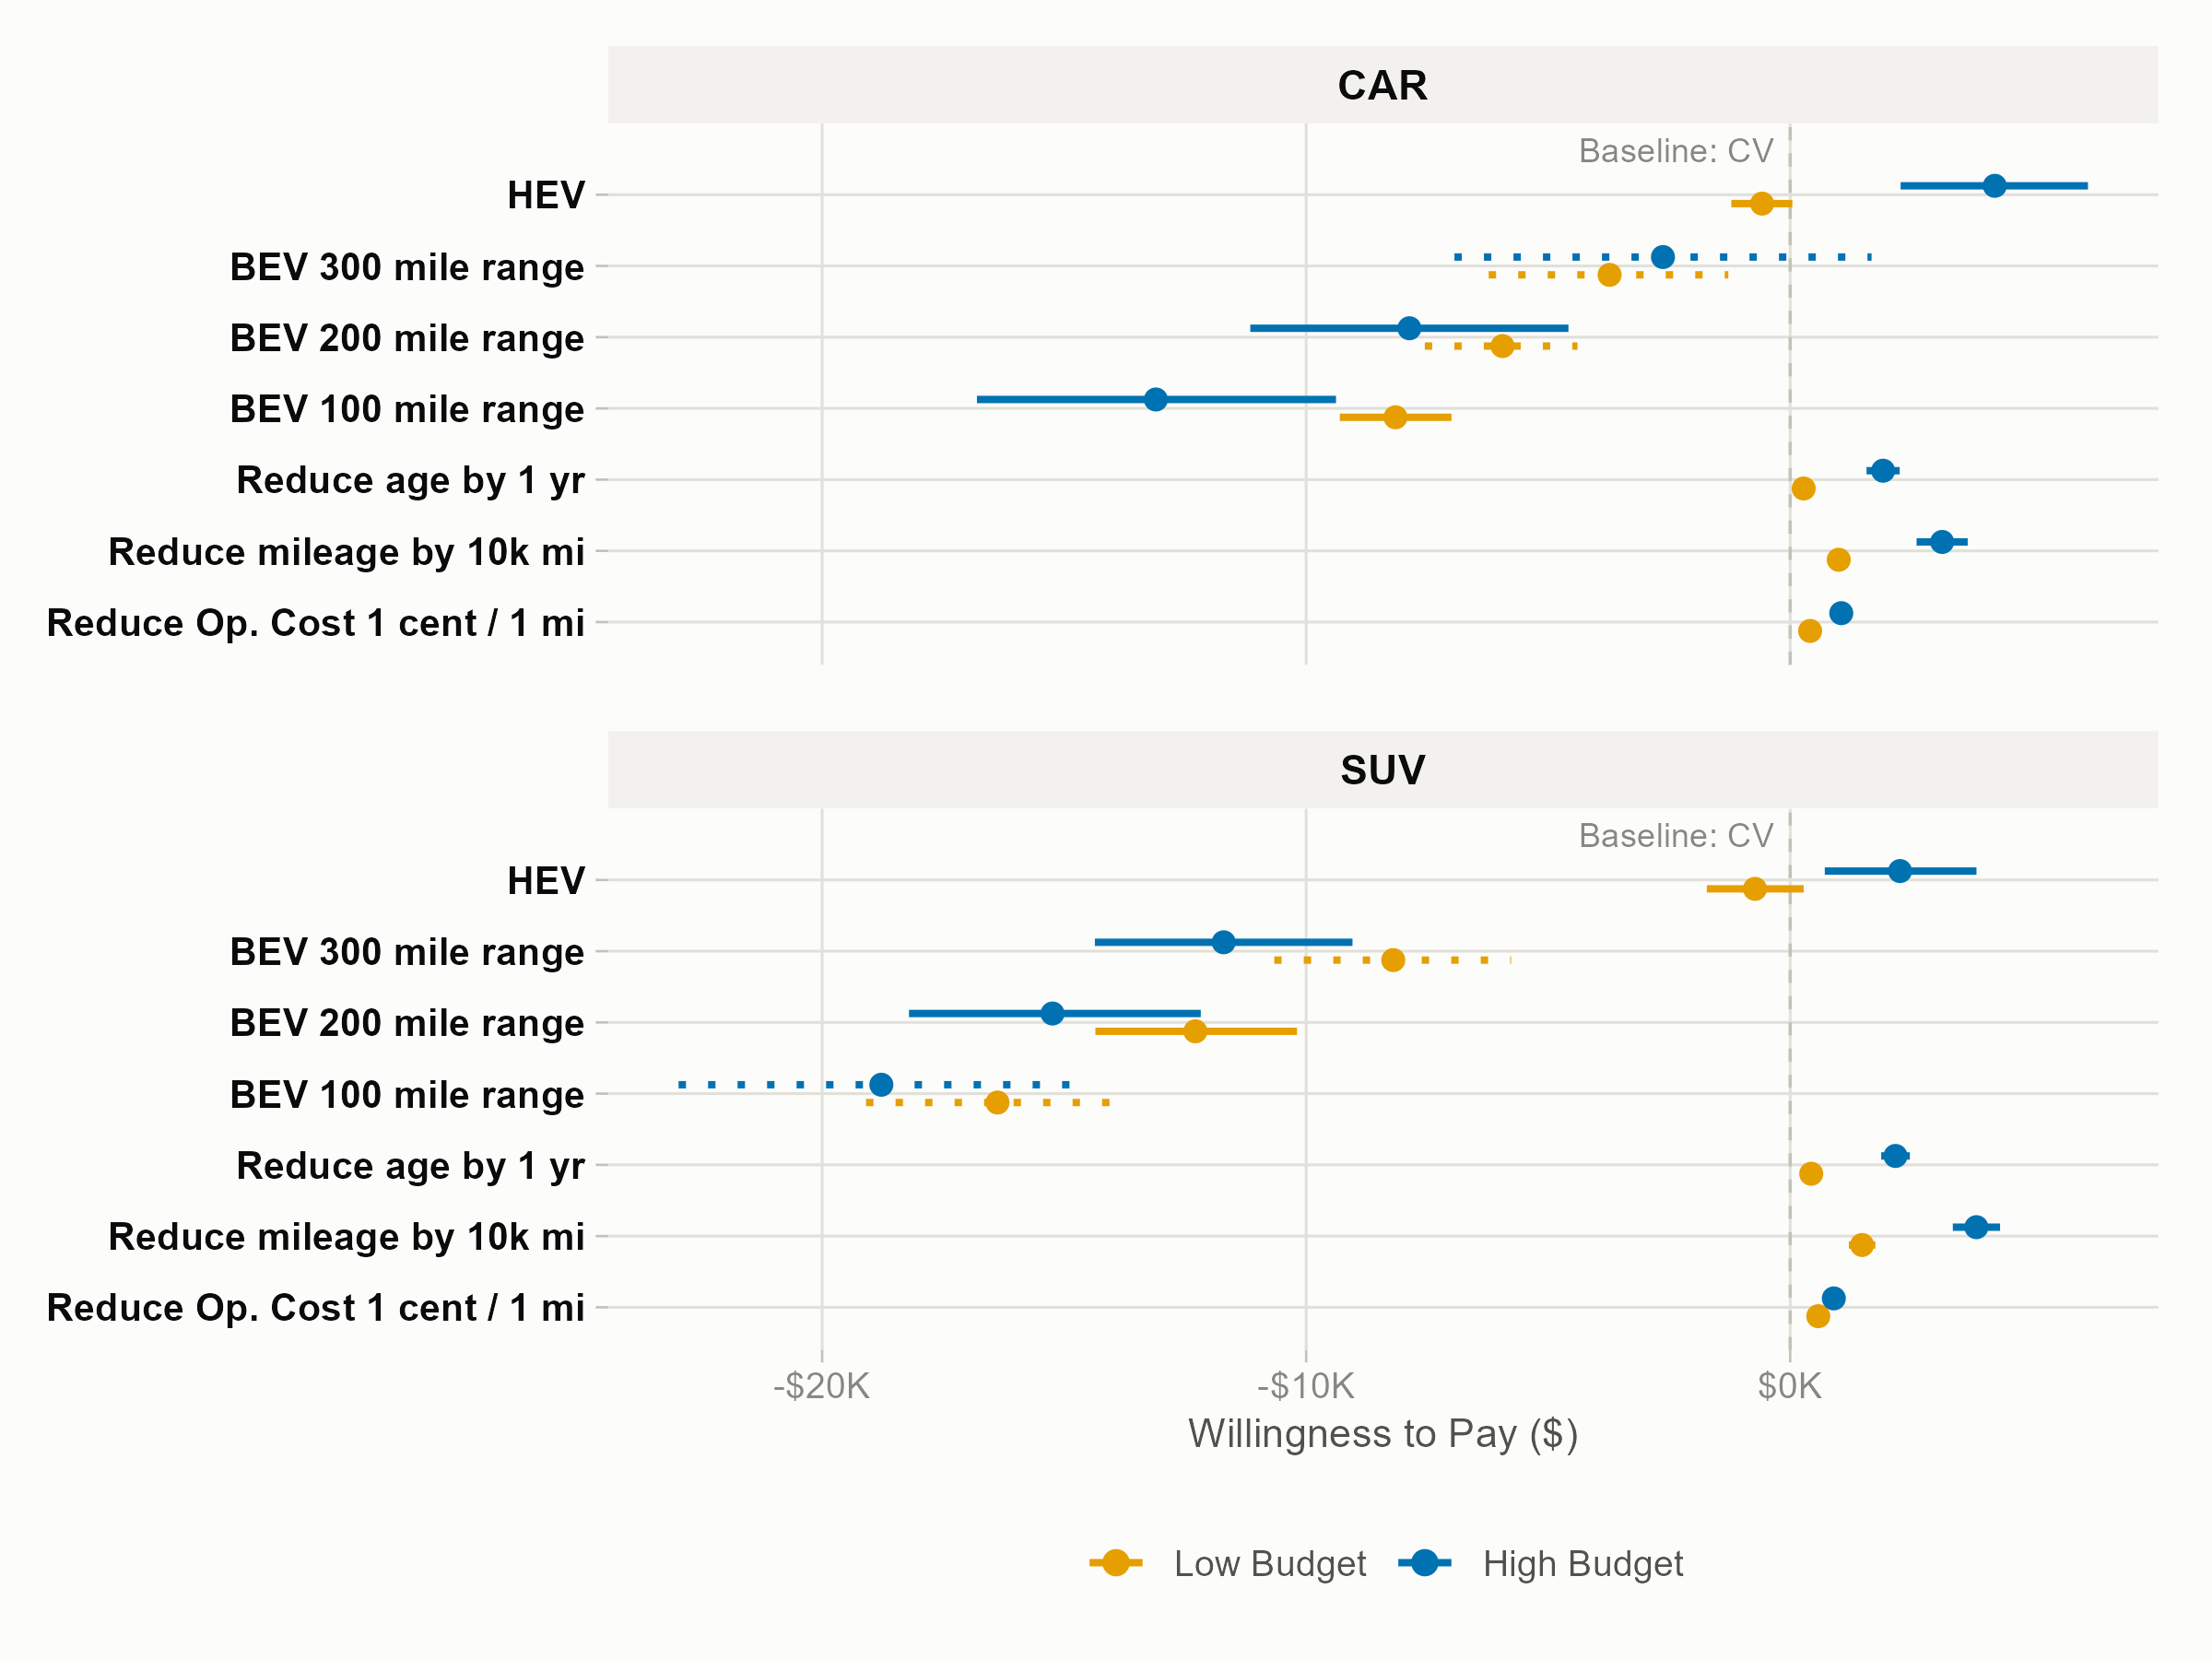
\includegraphics[width=\textheight]{images/vehicle_analysis/wtp_plot_vehicle_attributes.png}
    \caption{Willingness to pay (WTP) for vehicle attributes by vehicle segment and budget tier, relative to a conventional vehicle. Points are mean WTP (in thousands of dollars) and bars are 95\% simulation intervals. BEV values combine the powertrain and range coefficients at 100, 200, and 300 miles, with vehicle age, mileage, and operating cost held equal to the conventional vehicle; solid intervals are within the range shown to that segment in the choice experiment and dotted intervals are extrapolated beyond it. Age, mileage, and operating-cost values are for a one-year, 10,000-mile, and one-cent-per-mile reduction, respectively.}
    \label{fig:wtp_vehicle_attributes}
\end{figure}
\end{landscape}

\subsection{Used BEVs and HEVs Compared with Conventional Counterparts}
\label{subsec:wtp_vehicle_comparisons}

To compare stated WTP with observed pricing, matched pairs of existing alternative fuel vehicles (AFVs) sharing a common conventional counterpart were identified in the used market, following the logic of \textcite{helveston2014ChinaUSPreferences}, which argued that competitiveness is set by a vehicle's full attribute bundle relative to a specific counterpart rather than by powertrain alone. Real used-market listings were drawn from marketcheck.com for the year 2025. A pair was retained only if it had at least 200 listings between 2.5 and 3.5 years of vehicle age. Each pair was assigned to a budget-tier model by the mean price of its AFV: pairs with a mean AFV price at or below \$24,000 (cars) or \$30,000 (SUVs) were assigned to the low-budget model, and the rest to the high-budget model. These thresholds are the upper price bounds of the low-budget car and SUV design cells (\$20,000 and \$25,000) raised by 20\% to account for the higher prices of AFVs in the market.

Net WTP for each pair was simulated from the matched model in Table~\ref{table:mxl_results_vehicle}, using the simulation procedure in Section~\ref{section:method}. For a BEV,

\begin{equation}
\text{Net WTP}_{\text{BEV}} = \hat{\mu}_{\mathrm{BEV}} + \hat{\mu}_{\mathrm{range}} \cdot r_3 + \hat{\mu}_{\mathrm{cost}} \cdot \Delta c,
\label{eq:net_wtp}
\end{equation}

\noindent where $r_3 = r_0(1-\delta)^3$ is the new-vehicle range $r_0$ (in hundreds of miles) reduced at an assumed annual rate $\delta = 5\%$ to three years of age, and $\Delta c$ is the operating-cost differential between the powertrain of interest and its ICEV counterpart, computed per pair from EPA fuel-economy ratings (miles per gallon for the ICEV and HEV, kWh per 100 miles for the BEV) at \$3.18 per gallon of gasoline and \$0.17 per kWh of electricity. The differentials range from $-6.0$ to $-4.5$ cents per mile for the BEV pairs and from $-4.4$ to $-2.9$ for the HEV pairs. Both vehicles in a pair are three years old, so the age coefficient cancels. For an HEV, the range term is omitted, the powertrain coefficient is $\hat{\mu}_{\mathrm{HEV}}$, and the operating-cost term is retained. A pair is described as consistent with Net WTP when the observed premium lies within the 95\% interval, and as above or below it when the premium lies outside the interval.

Figures~\ref{fig:waterfall_wtp_bev} and~\ref{fig:waterfall_wtp_hev} compare the WTP-implied value of specific used vehicles with their observed prices. Five pairs met the listing threshold, each supported by between 378 and 16,989 listings: three BEV pairs (high-budget car, low-budget car, low-budget SUV) and two HEV pairs (high-budget car, high-budget SUV); no BEV pair was available for the high-budget SUV segment and no HEV pair for either low-budget segment. Bars show the contributions of powertrain, driving range (depreciated to three years), and operating cost to simulated Net WTP, the point and interval show Net WTP (mean and 95\% simulation interval), and the dashed line shows the observed mean price premium over the conventional counterpart.

For BEVs (Figure~\ref{fig:waterfall_wtp_bev}), the powertrain term is the largest negative contribution in every pair ($-\$10,375$ to $-\$20,485$). It is offset by driving range (+\$2,852 to +\$11,219, based on each vehicle's range depreciated to three years) and by operating cost (+\$1,839 to +\$6,297). Simulated Net WTP is negative for the low-budget car ($-\$5,685$; 95\% interval $-\$6,824$ to $-\$4,564$) and the low-budget SUV ($-\$8,190$; $-\$10,149$ to $-\$6,238$), and is not distinguishable from zero for the high-budget car ($-\$800$; $-\$3,972$ to +\$2,344).

Observed premiums differ sharply across the three BEV pairs. The high-budget car BEV is priced at approximately parity with its conventional counterpart ($-\$68$), which is consistent with its Net WTP interval. The two lower-budget BEVs are priced above their conventional counterparts (low-budget car: +\$8,585; low-budget SUV: +\$5,962), whereas the Net WTP estimates imply a discount. The observed premiums exceed Net WTP by roughly \$14,300 and \$14,200, respectively, and lie well above the upper ends of the intervals.

For HEVs (Figure~\ref{fig:waterfall_wtp_hev}), the powertrain term is positive (+\$4,240 for the high-budget car; +\$2,271 for the high-budget SUV), and operating cost adds +\$4,640 and +\$2,581, giving Net WTP of +\$8,879 (95\% interval \$6,943 to \$10,799) and +\$4,850 (\$3,153 to \$6,543). In the high-budget car segment the observed premium (+\$1,945) lies well below the interval, roughly \$6,900 below mean Net WTP. In the high-budget SUV segment the observed premium (+\$7,987) lies above the interval, roughly \$3,100 above mean Net WTP.

Net WTP depends on the assumed fuel prices through the operating-cost differential. Figures~\ref{fig:gas_sensitivity_bev} and~\ref{fig:gas_sensitivity_hev} (Appendix~\ref{app:gas_sensitivity}) recompute each comparison for gasoline prices from \$2.50 to \$5.00 per gallon, holding electricity at \$0.17 per kWh; a higher gasoline price raises Net WTP for every pair by widening the fuel-cost advantage of the alternative powertrain. For three of the five pairs the conclusion does not change: the observed premiums for both lower-budget BEVs and the high-budget car HEV lie outside the Net WTP interval at every gasoline price (above it for the BEVs, below it for the HEV). The high-budget car BEV premium is consistent with Net WTP at approximately \$2.60 to \$4.20 per gallon, and Net WTP is distinguishable from zero only above about \$4.30. The high-budget SUV HEV premium lies above the interval except at roughly \$4.85 and higher, making it the result most sensitive to the fuel-price assumption. Each 1 cent per mile change in the operating-cost differential changes Net WTP by \$412 to \$1,054, depending on the model (Table~\ref{table:mxl_results_vehicle}).

Two limitations apply. First, the comparison rests on five pairs and cannot be generalized to the used market as a whole. Second, each AFV and its conventional counterpart are different models of similar vehicles that differ in powertrain, so Net WTP, which covers powertrain, range, and operating cost only, omits other differences that observed premiums also reflect, such as incentives, and supply-side factors. The implications are discussed in Section~\ref{section:discussion}.

\begin{figure}[pos=H]
    \centering
    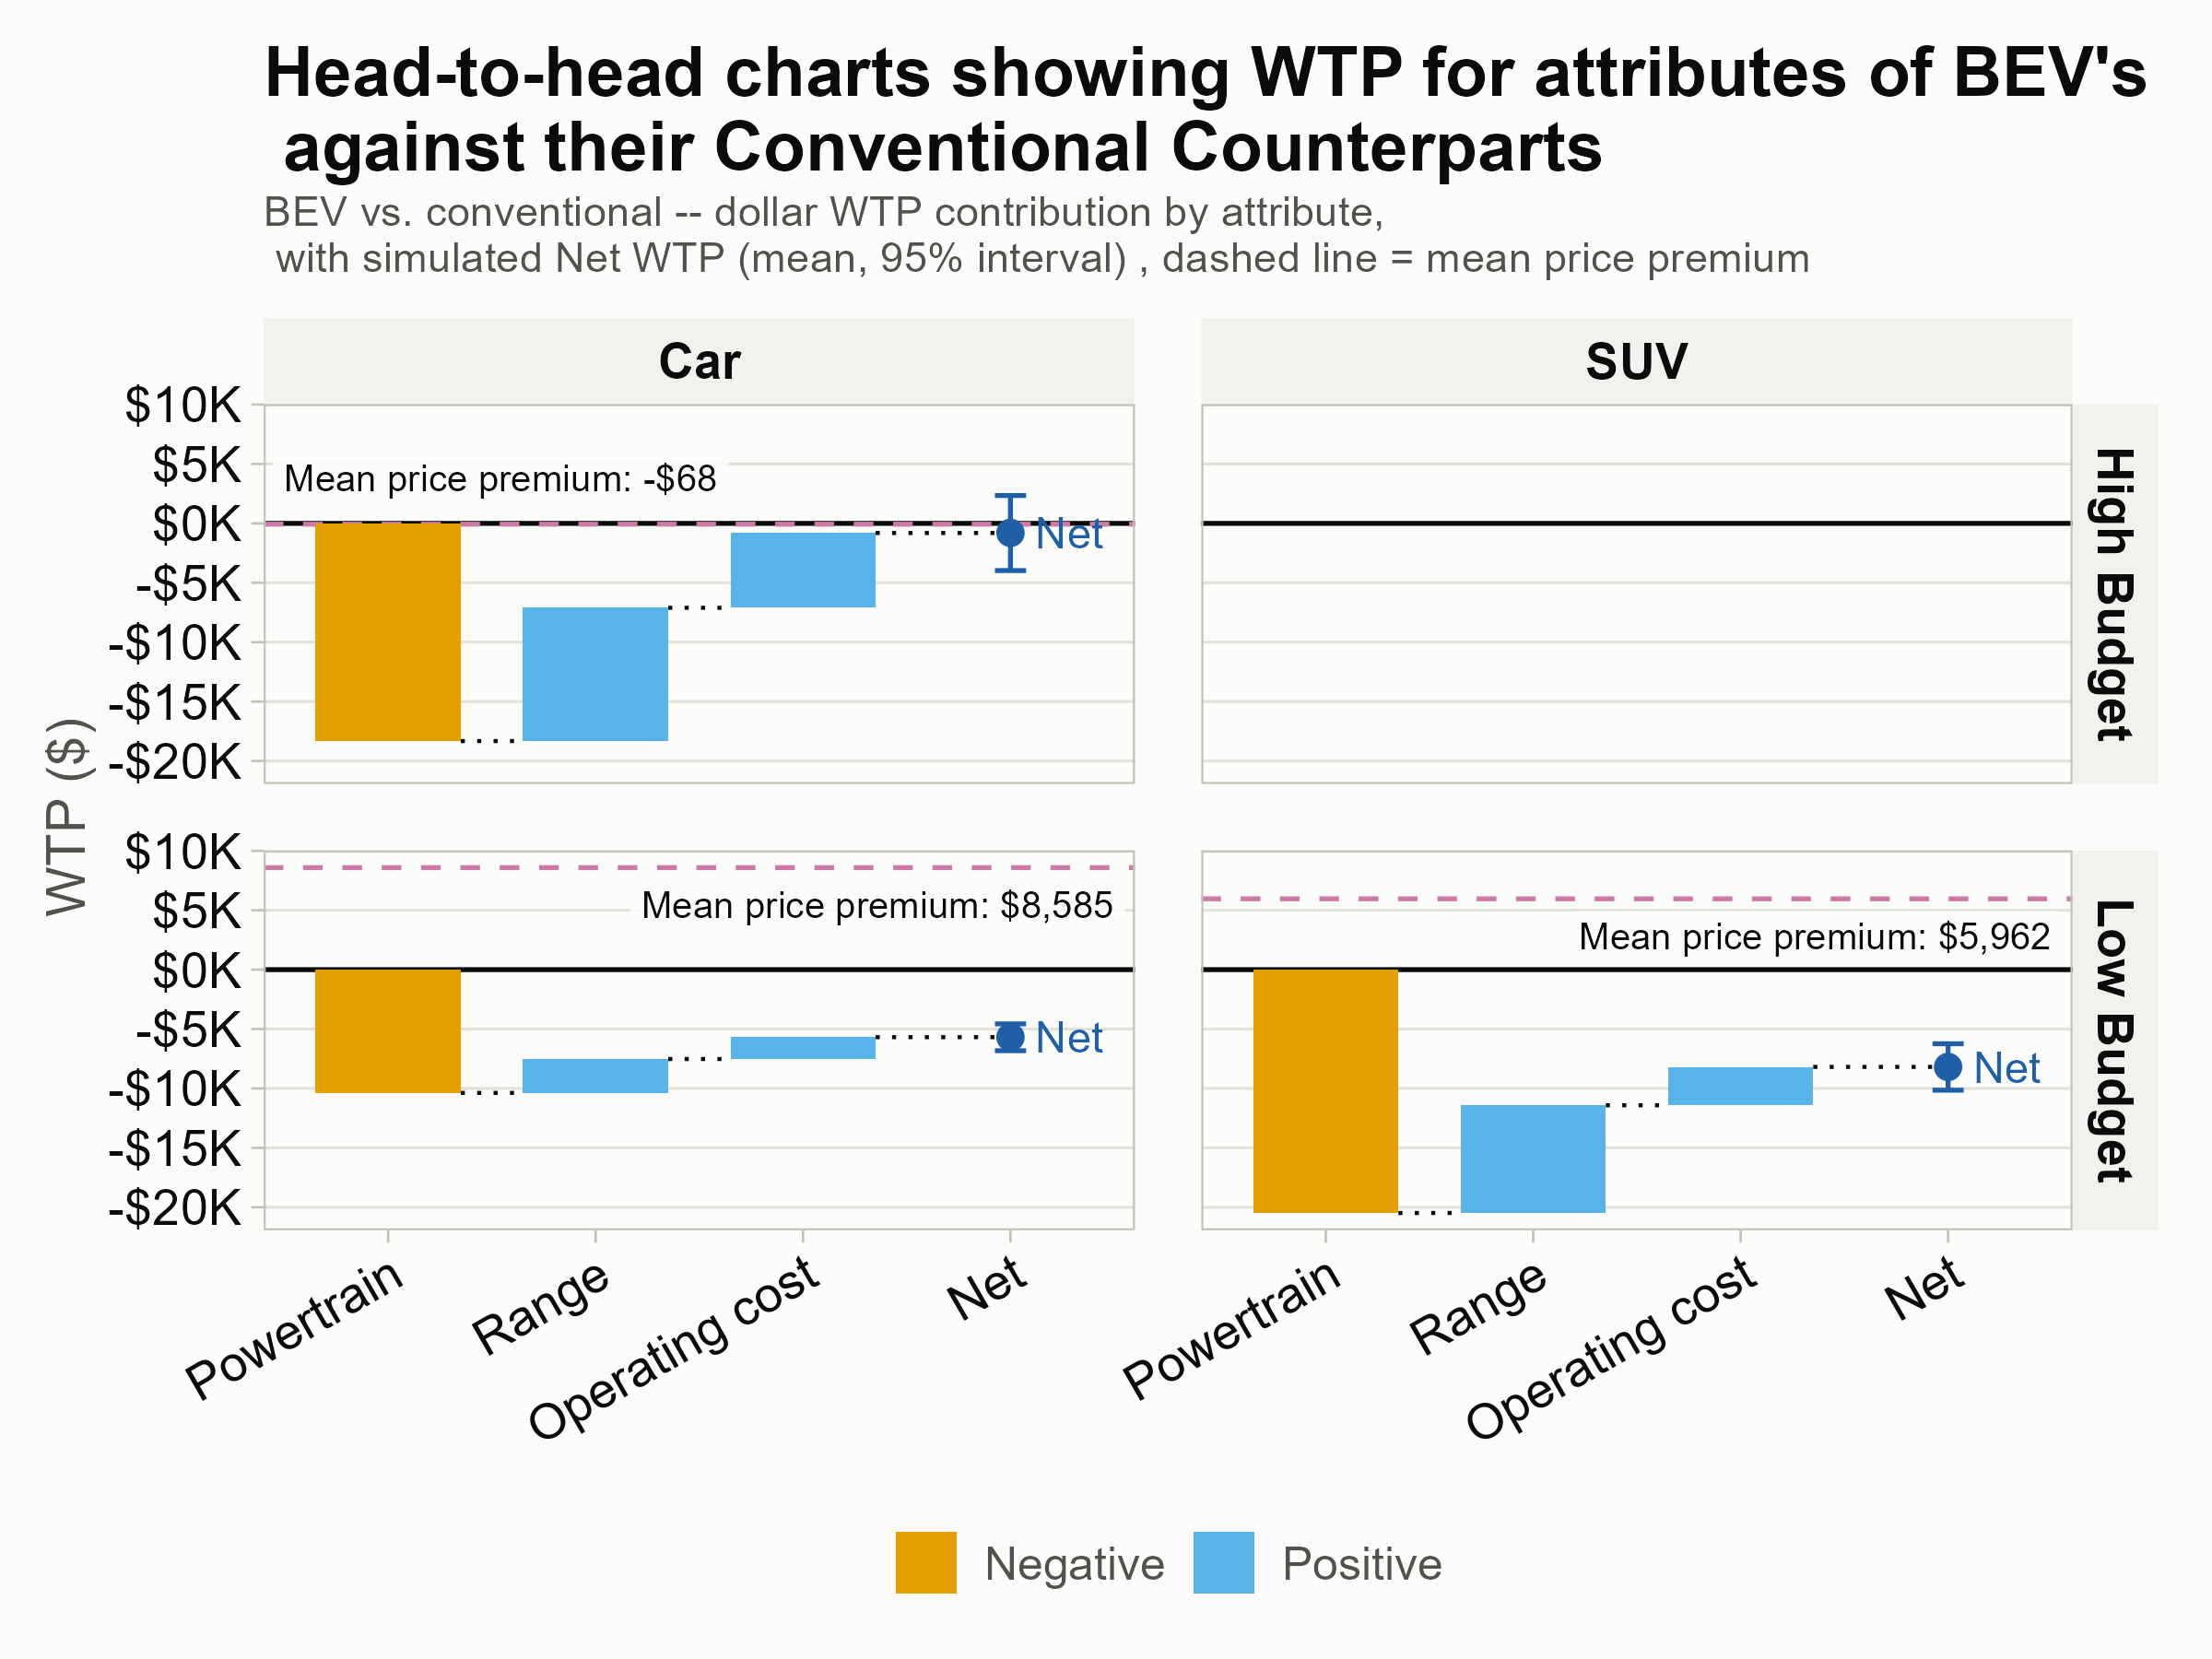
\includegraphics[width=0.85\textwidth]{images/vehicle_analysis/waterfall_wtp_bev.png}
    \caption{Simulated Net WTP versus observed price premium: BEV pairs. Bars decompose WTP (powertrain, driving range, and operating cost) for real BEVs relative to each vehicle's closest conventional counterpart, by vehicle segment and budget tier. The blue point and error bar show simulated Net WTP (mean, 95\% interval); the dashed line is the observed mean price premium (or discount) at approximately three years of age. Operating-cost contributions use EPA-based fuel-cost differentials at \$3.18 per gallon of gasoline and \$0.17 per kWh of electricity. No matched BEV pair met the sample-size threshold for the high-budget SUV segment.}
    \label{fig:waterfall_wtp_bev}
\end{figure}

\begin{figure}[pos=H]
    \centering
    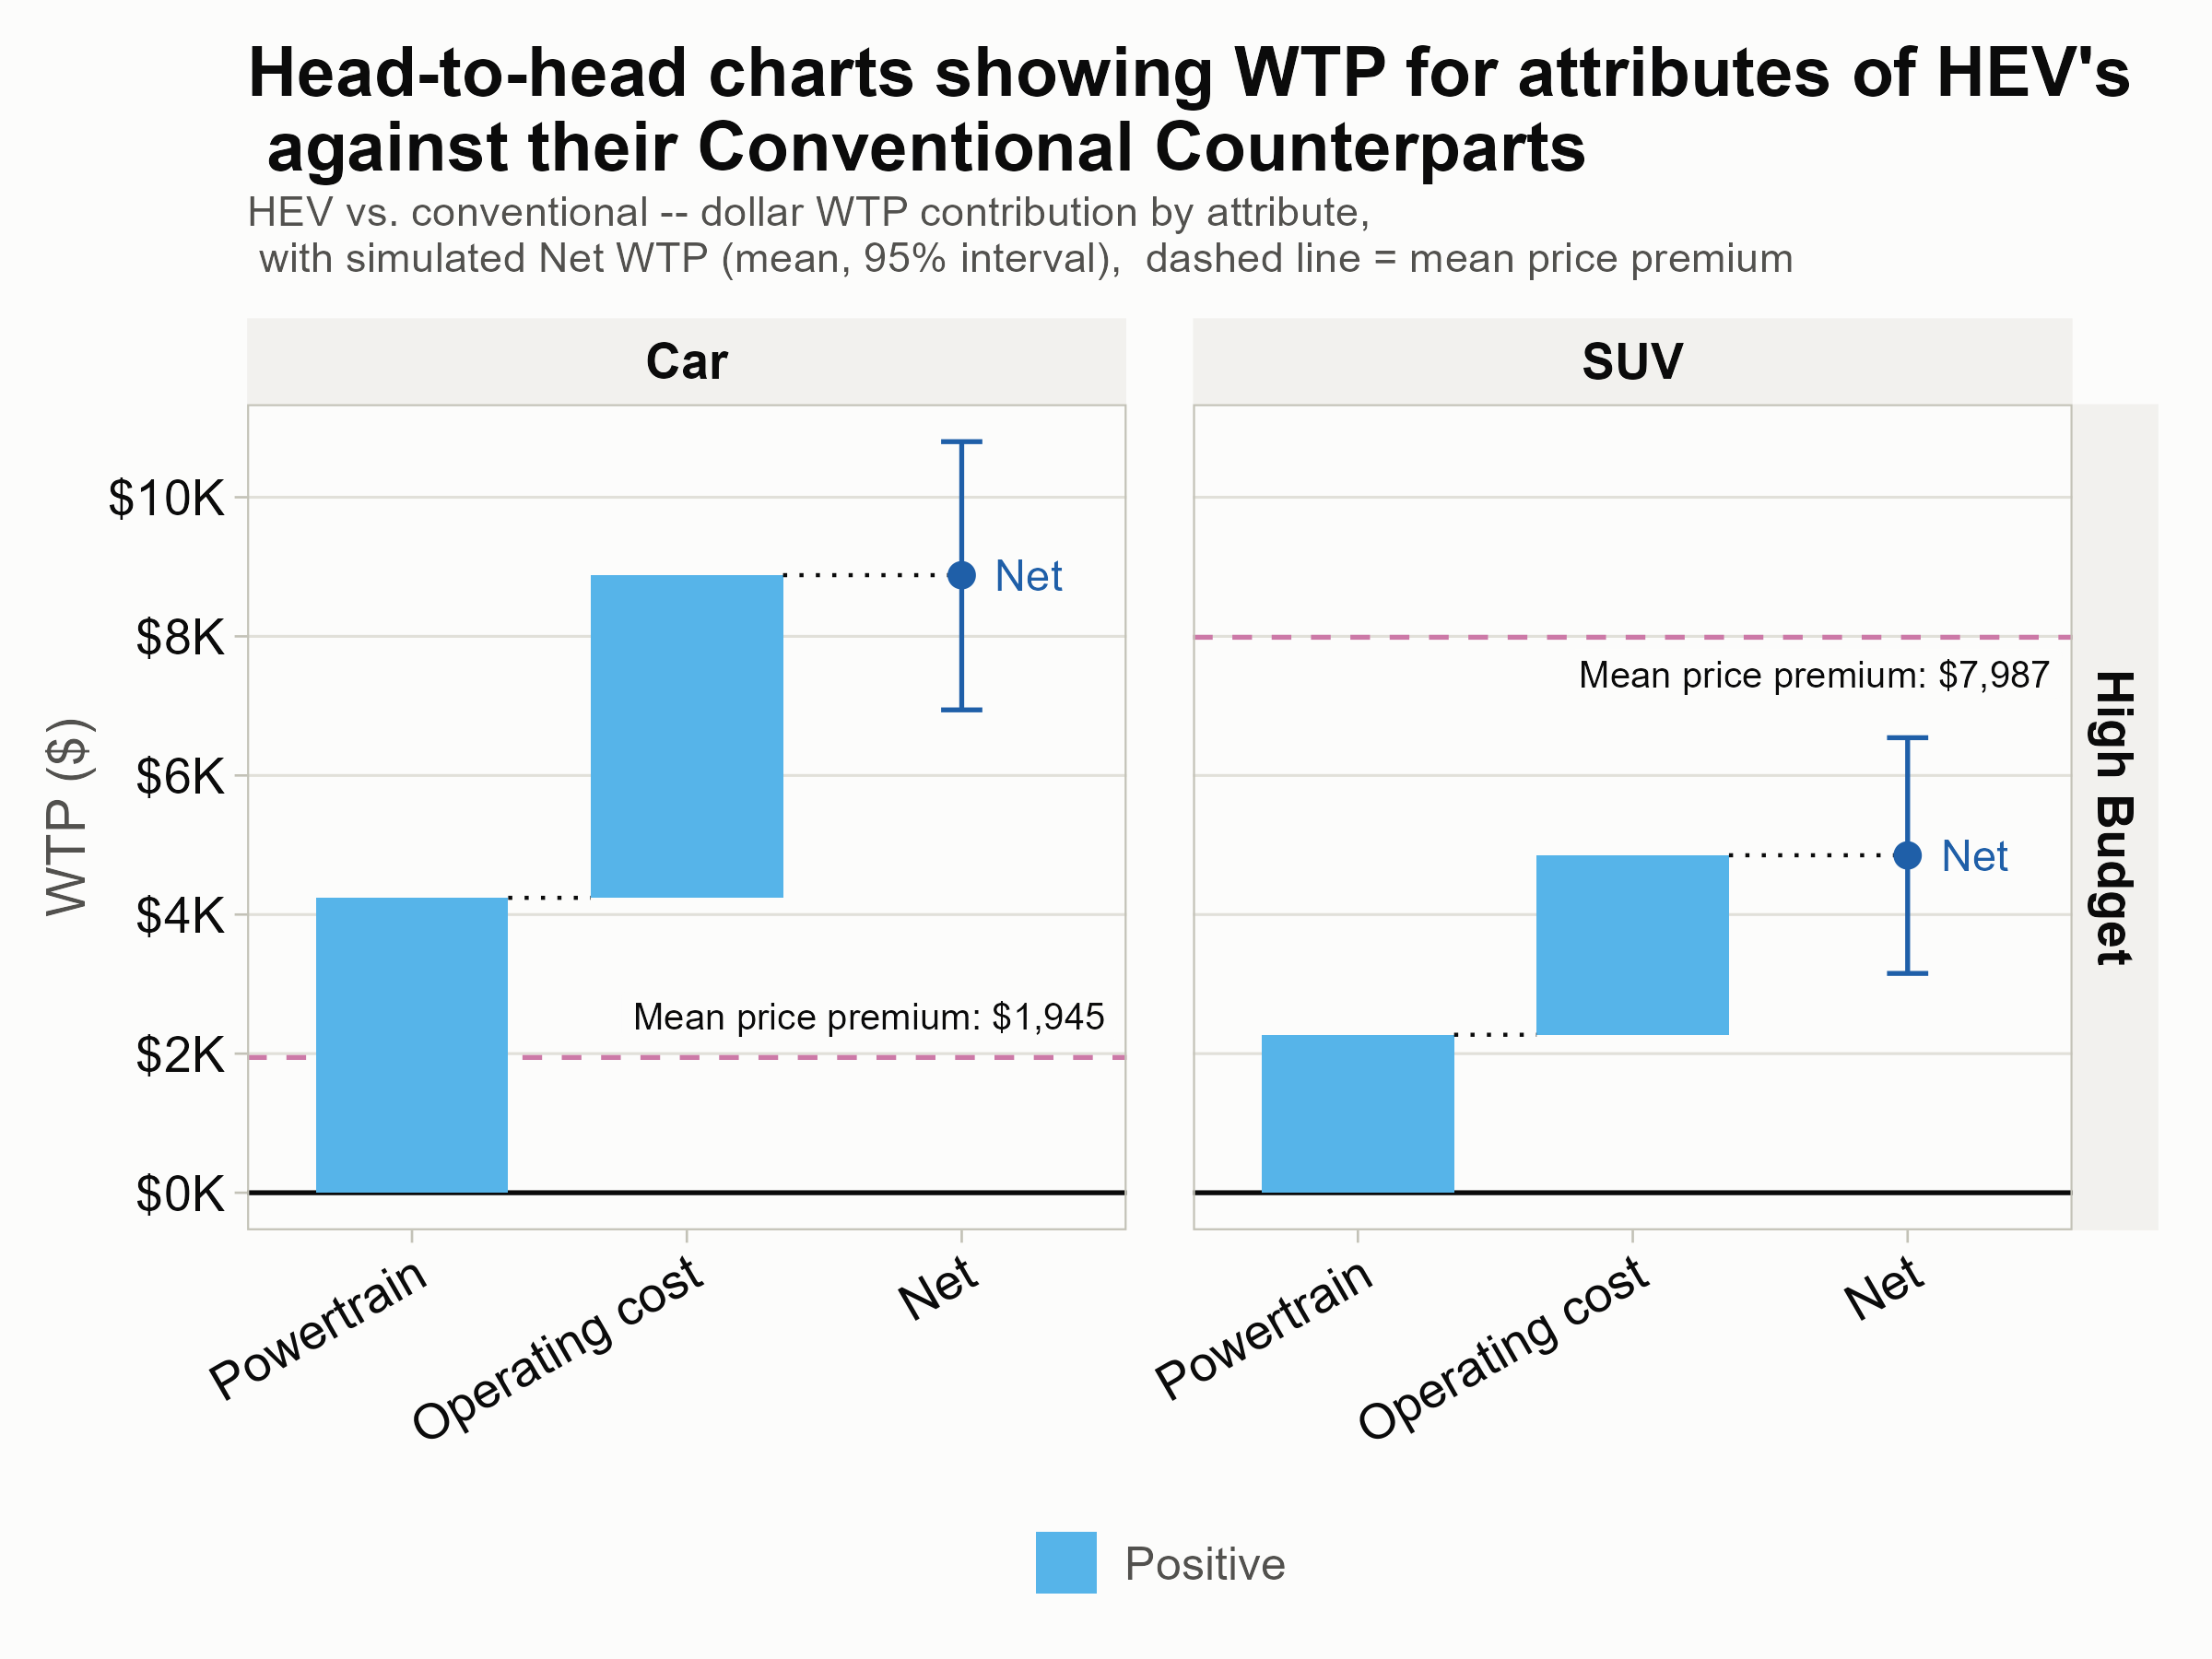
\includegraphics[width=0.85\textwidth]{images/vehicle_analysis/waterfall_wtp_hev.png}
    \caption{Simulated Net WTP versus observed price premium: HEV pairs. Bars decompose WTP (powertrain and operating cost) for real HEVs relative to each vehicle's closest conventional counterpart, by vehicle segment and budget tier. The blue point and error bar show simulated Net WTP (mean, 95\% interval); the dashed line is the observed mean price premium at approximately three years of age. Operating-cost contributions use EPA-based fuel-cost differentials at \$3.18 per gallon of gasoline. No matched HEV pair met the sample-size threshold in either low-budget segment.}
    \label{fig:waterfall_wtp_hev}
\end{figure}





\section{Discussion and Policy Implications}
\label{section:discussion}

Past U.S. incentives for electric vehicles were designed mainly around the new-vehicle market, and the used-vehicle incentives that followed were limited to lower-priced vehicles (a price cap of about \$25,000) and to buyers below income thresholds. Although such programs are no longer available, the estimates indicate how well incentives of this design fit the used-vehicle market.

\subsection{Fit of price-capped incentives}

The results largely support a price cap of this kind. The high-budget car segment, whose vehicles are priced above such a cap, is already close to price parity with conventional vehicles: the high-budget car BEV is priced near its conventional counterpart, consistent with its Net WTP interval (Section~\ref{subsec:wtp_vehicle_comparisons}), and its WTP penalty is not distinguishable from zero at 300 miles (an extrapolation beyond the design range). Subsidizing this segment may therefore offer less additional benefit, although stated WTP for BEVs remains negative at the ranges tested. The lower-budget segments, which fall largely under the cap (the low-budget SUV pair is slightly above it), have negative Net WTP and observed premiums well above it, and are where support is most likely to change purchases. Consistent with \textcite{robersonNotAllSubsidies2022}, incentive structure matters as much as magnitude: buyers are reported to value immediate rebates well above equivalent tax credits, most strongly among the lower-income, lower-budget, and used-vehicle buyers who dominate this market.

\subsection{Interpreting the comparison with real-market prices}

The comparison in Section~\ref{subsec:wtp_vehicle_comparisons} does not show uniform overpricing of used BEVs: observed premiums exceed Net WTP in the two lower-budget pairs but not in the high-budget car pair. Because Net WTP is a population mean and a minority of buyers value BEVs positively (Section~\ref{subsec:mxl_heterogeneity}), prices above it are not necessarily unsellable; demand at those prices is concentrated in the upper tail of the distribution. Repricing or point-of-sale support are therefore the candidate responses where observed premiums sit well above WTP. The hybrid pairs differ by segment and the SUV result is sensitive to fuel prices, and with five pairs in total these comparisons illustrate segment-level contrasts rather than characterize the used-vehicle market as a whole.

\subsection{Non-price instruments and segment-aware policy}

Uncertainty about battery state of health is a plausible source of part of the BEV valuation gap \parencite{trd2024usedEV_concerns}. Measures that make battery condition observable, such as a standard health report at listing or warranty cover that transfers on resale \parencite{trd2019batterywarranty}, target that source and would plausibly cost less in public funds than a point-of-sale subsidy. The results thus favor segment-aware policy: point-of-sale support for BEVs in the lower-budget segments where observed prices exceed WTP, attention to HEV adoption in the high-budget car segment, where observed prices sit below WTP (though HEV results depend on the operating-cost levels shown), and measures to close the battery-health information gap.


\section{Conclusion}
\label{section:conclusion}

This study estimated willingness to pay (WTP) for powertrain type and vehicle attributes among 2,254 prospective used-vehicle buyers using four mixed logit models by vehicle segment and budget tier, and compared the estimates with observed prices for matched real vehicles. A used BEV carries a significant WTP penalty relative to an equivalent conventional vehicle in every model, and the penalty narrows as driving range increases. Within the ranges shown to respondents the penalty is distinguishable from zero in every segment; the only interval that includes zero is the high-budget car at 300 miles, an extrapolation beyond that cell's design range. HEV powertrains command a significant premium only among high-budget buyers. Comparison with matched real vehicles is mixed: two lower-budget BEVs are priced well above WTP-implied values, a high-budget car BEV is priced near parity, and hybrid prices fall below WTP for a high-budget car and above it for a high-budget SUV.

These results carry three implications for used-BEV market development. First, used BEVs are not at price parity with conventional vehicles for most prospective buyers, and the segments where listed prices most exceed WTP (low-budget car and SUV) are those where repricing or a point-of-sale incentive would matter most. Second, range is the lever most clearly associated with narrowing the gap, but the only estimate whose interval includes zero lies beyond the ranges respondents evaluated, so it should be tested directly. Third, measures that make battery condition observable, such as standardized health reports and transferable warranties, are a plausible complement to price-based support.

The findings should be read with several limitations in mind. The analysis rests on stated rather than revealed preferences, and because the WTP-space models scale every attribute by a single price parameter, any hypothetical bias in price sensitivity propagates into every WTP estimate; its direction is uncertain. The sample was drawn from online research panels and may over-represent respondents comfortable with new technology, which could bias BEV valuations upward. The two panels are pooled in the models without a panel indicator, and budget is self-reported, so differences between budget tiers also reflect the price and range levels each design cell displayed; differences across segments and tiers were not formally tested. The mixed logit specification assumes continuous, unimodal normal mixing distributions, which may hide a distinct group of firm BEV rejecters. The powertrain attribute had three levels and excluded plug-in hybrids, and battery state of health was not varied in this experiment. The real-market comparison rests on five matched pairs, observed asking prices, a single vehicle age (approximately three years), and assumed range depreciation (5\% per year) and fuel prices, and some BEV pairs' mean prices lie above the price ranges shown in the corresponding design cells.

Future research could (i) add a plug-in-hybrid level to estimate PHEV WTP directly; (ii) estimate a latent-class specification to test whether the heterogeneity reflects a small number of distinct preference segments; (iii) link stated preferences to revealed transaction data, for example by matching respondents' subsequent purchases to dealer or DMV records, and broaden the real-market comparison to more pairs and vehicle ages; (iv) jointly estimate the vehicle and battery-health experiments to combine battery state-of-health penalties with the age- and mileage-driven depreciation identified here; and (v) exploit the attitudinal, knowledge, and sociodemographic variables collected in the survey but not used in this study to segment respondents further.

\section*{Acknowledgments and Disclaimers}

This study was funded by the National Institute of Standards and Technology (NIST) (grant number:70NANB25H110-0). The NIST Research Protections Office and the Office of Human Research of George Washington University determined this project meets the criteria for exempt human subjects research.

Certain equipment, instruments, software, or materials, commercial or non-commercial, are identified in this paper in order to specify the experimental procedure adequately. Such identification does not imply recommendation or endorsement of any product or service by NIST, nor does it imply that the materials or equipment identified are necessarily the best available for the purpose.

\section*{Declaration of Generative AI and AI-Assisted Technologies in the Manuscript Preparation Process}

During the preparation of this work the authors used Claude (Anthropic) in order to assist with grammar checking, language improvement, and table formatting. After using this tool, the authors reviewed and edited the content as needed and take full responsibility for the content of the published article.



\appendix

\section{Sensitivity of Net WTP to Gasoline Price}
\label{app:gas_sensitivity}

\begin{figure}[pos=H]
    \centering
    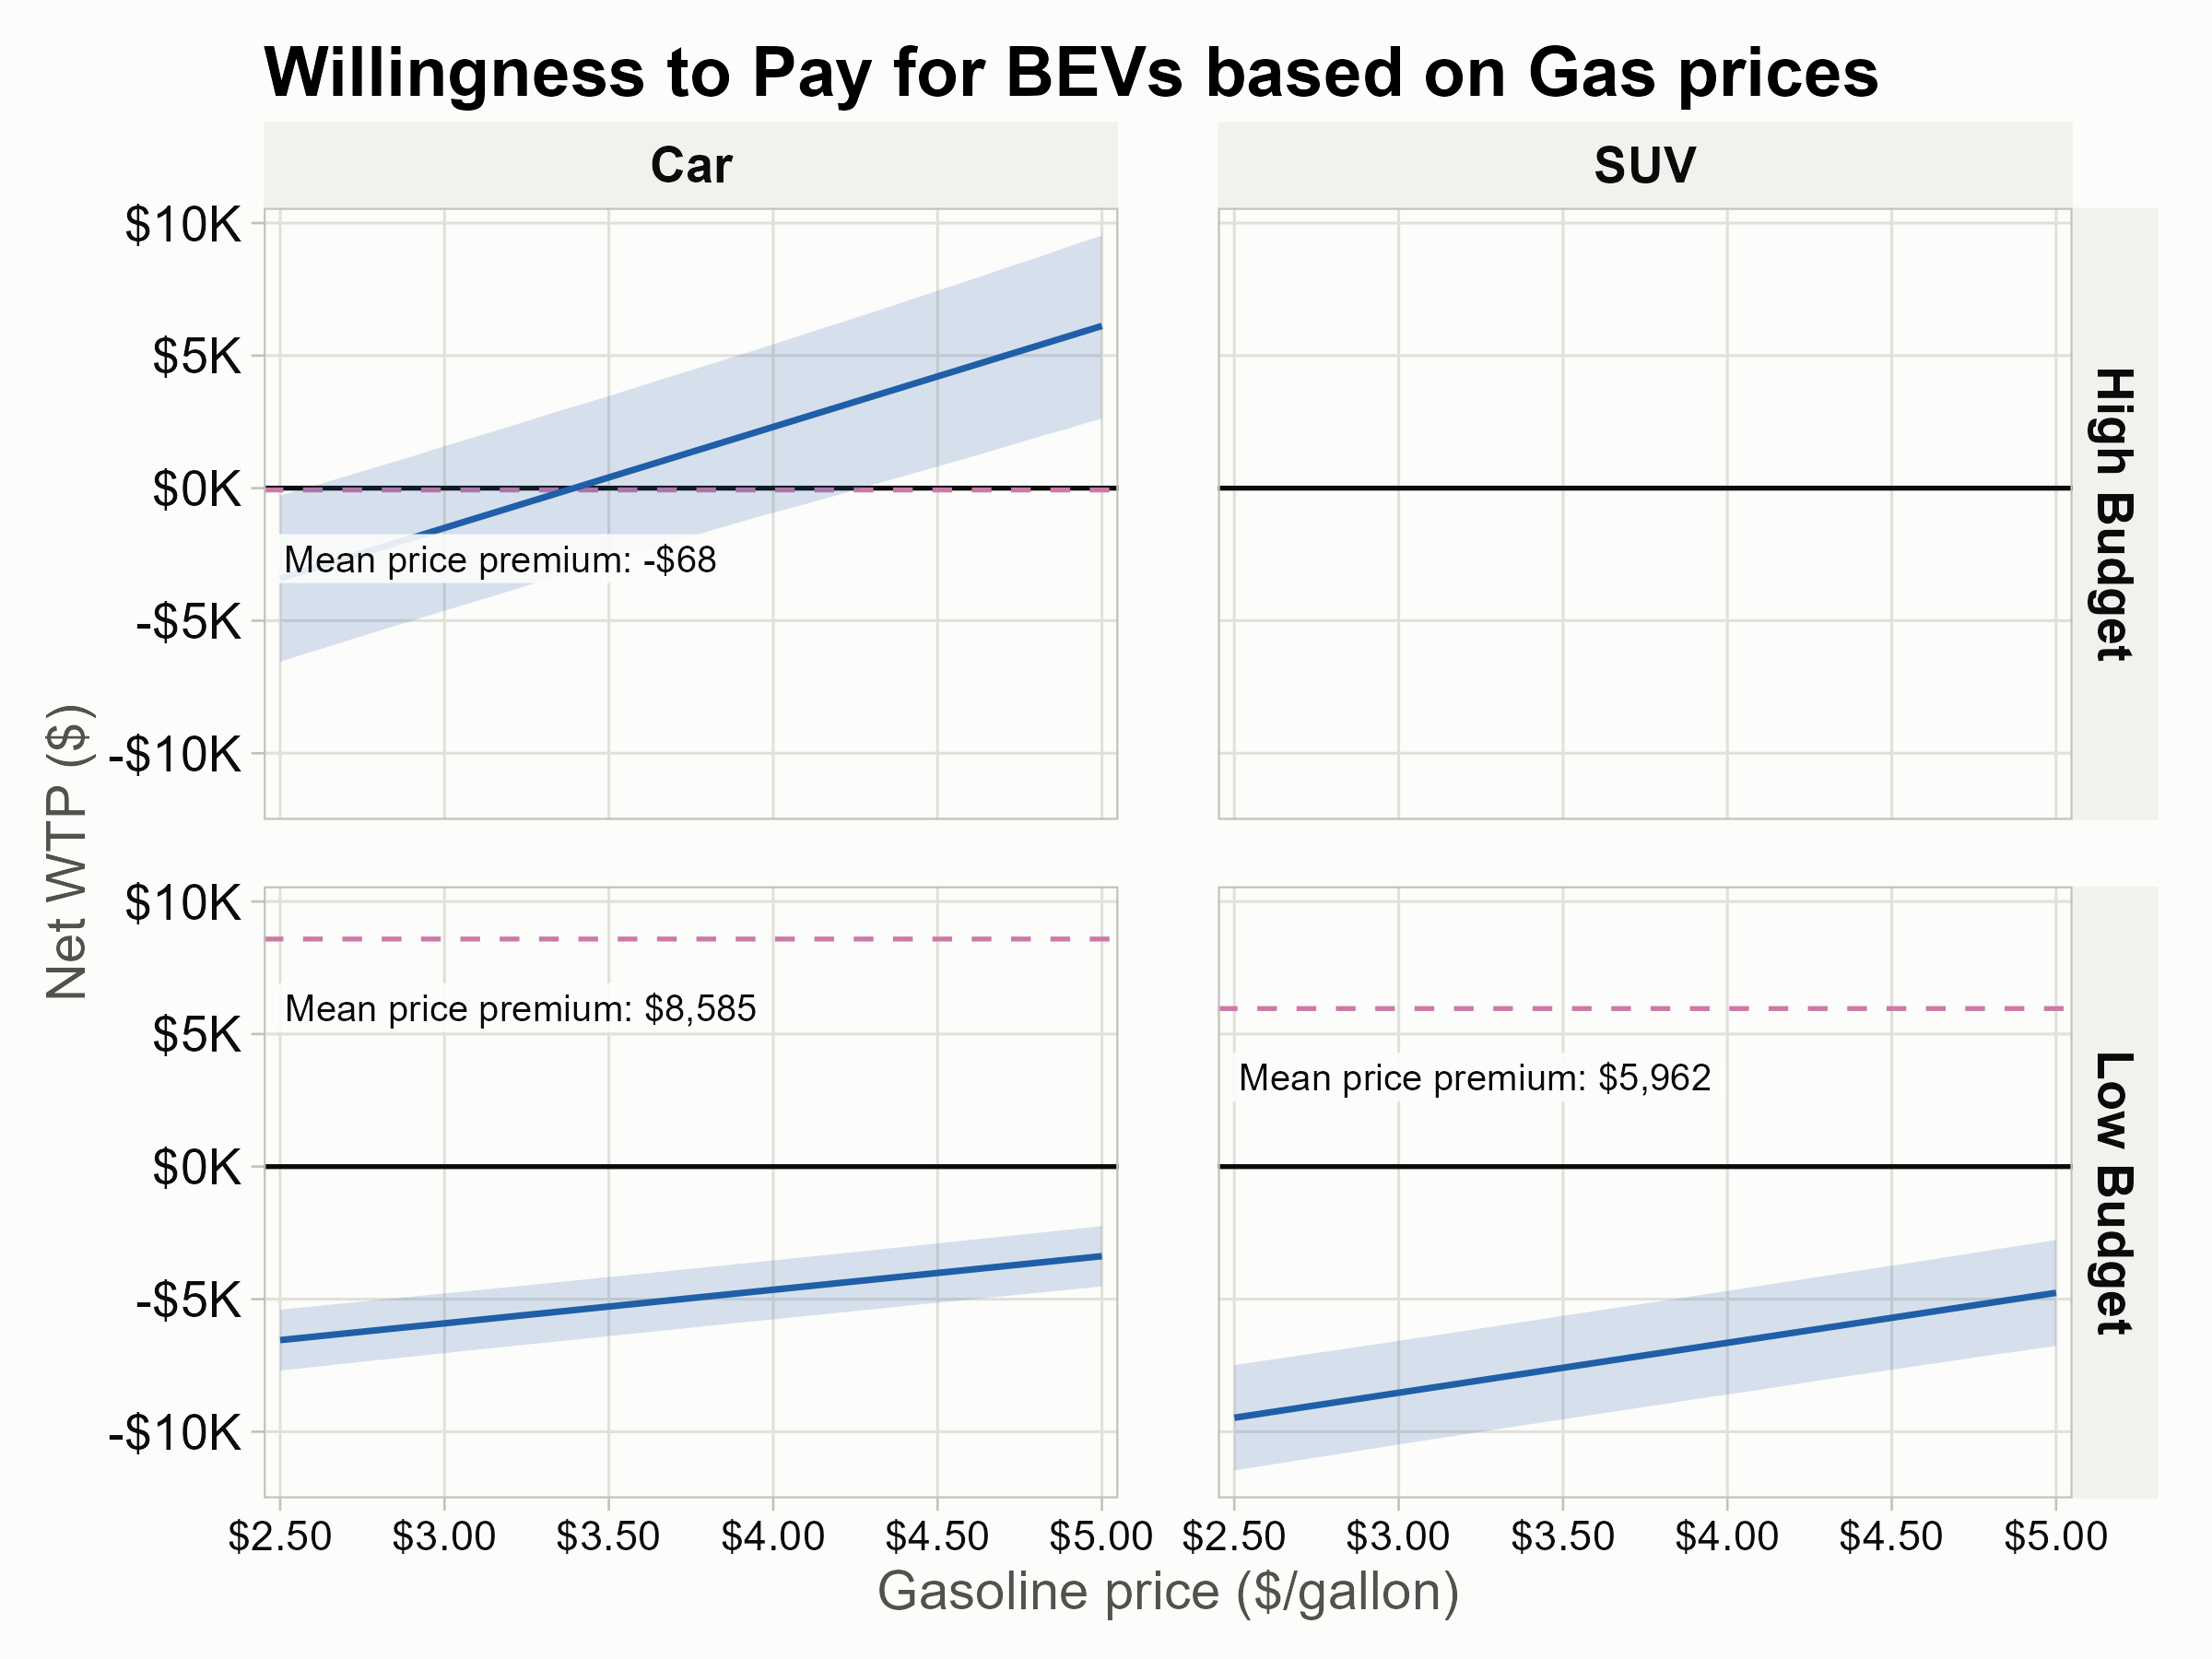
\includegraphics[width=0.85\textwidth]{images/vehicle_analysis/gas_price_sensitivity_bev.png}
    \caption{Net WTP versus gasoline price: BEV pairs. The blue line and band show simulated Net WTP (mean, 95\% interval) as the gasoline price varies from \$2.50 to \$5.00 per gallon, holding electricity at \$0.17 per kWh; the dashed line is the observed mean real-market price premium (or discount) at approximately three years of age. No matched BEV pair meeting the sample-size threshold was available for the high-budget SUV segment.}
    \label{fig:gas_sensitivity_bev}
\end{figure}

\begin{figure}[pos=H]
    \centering
    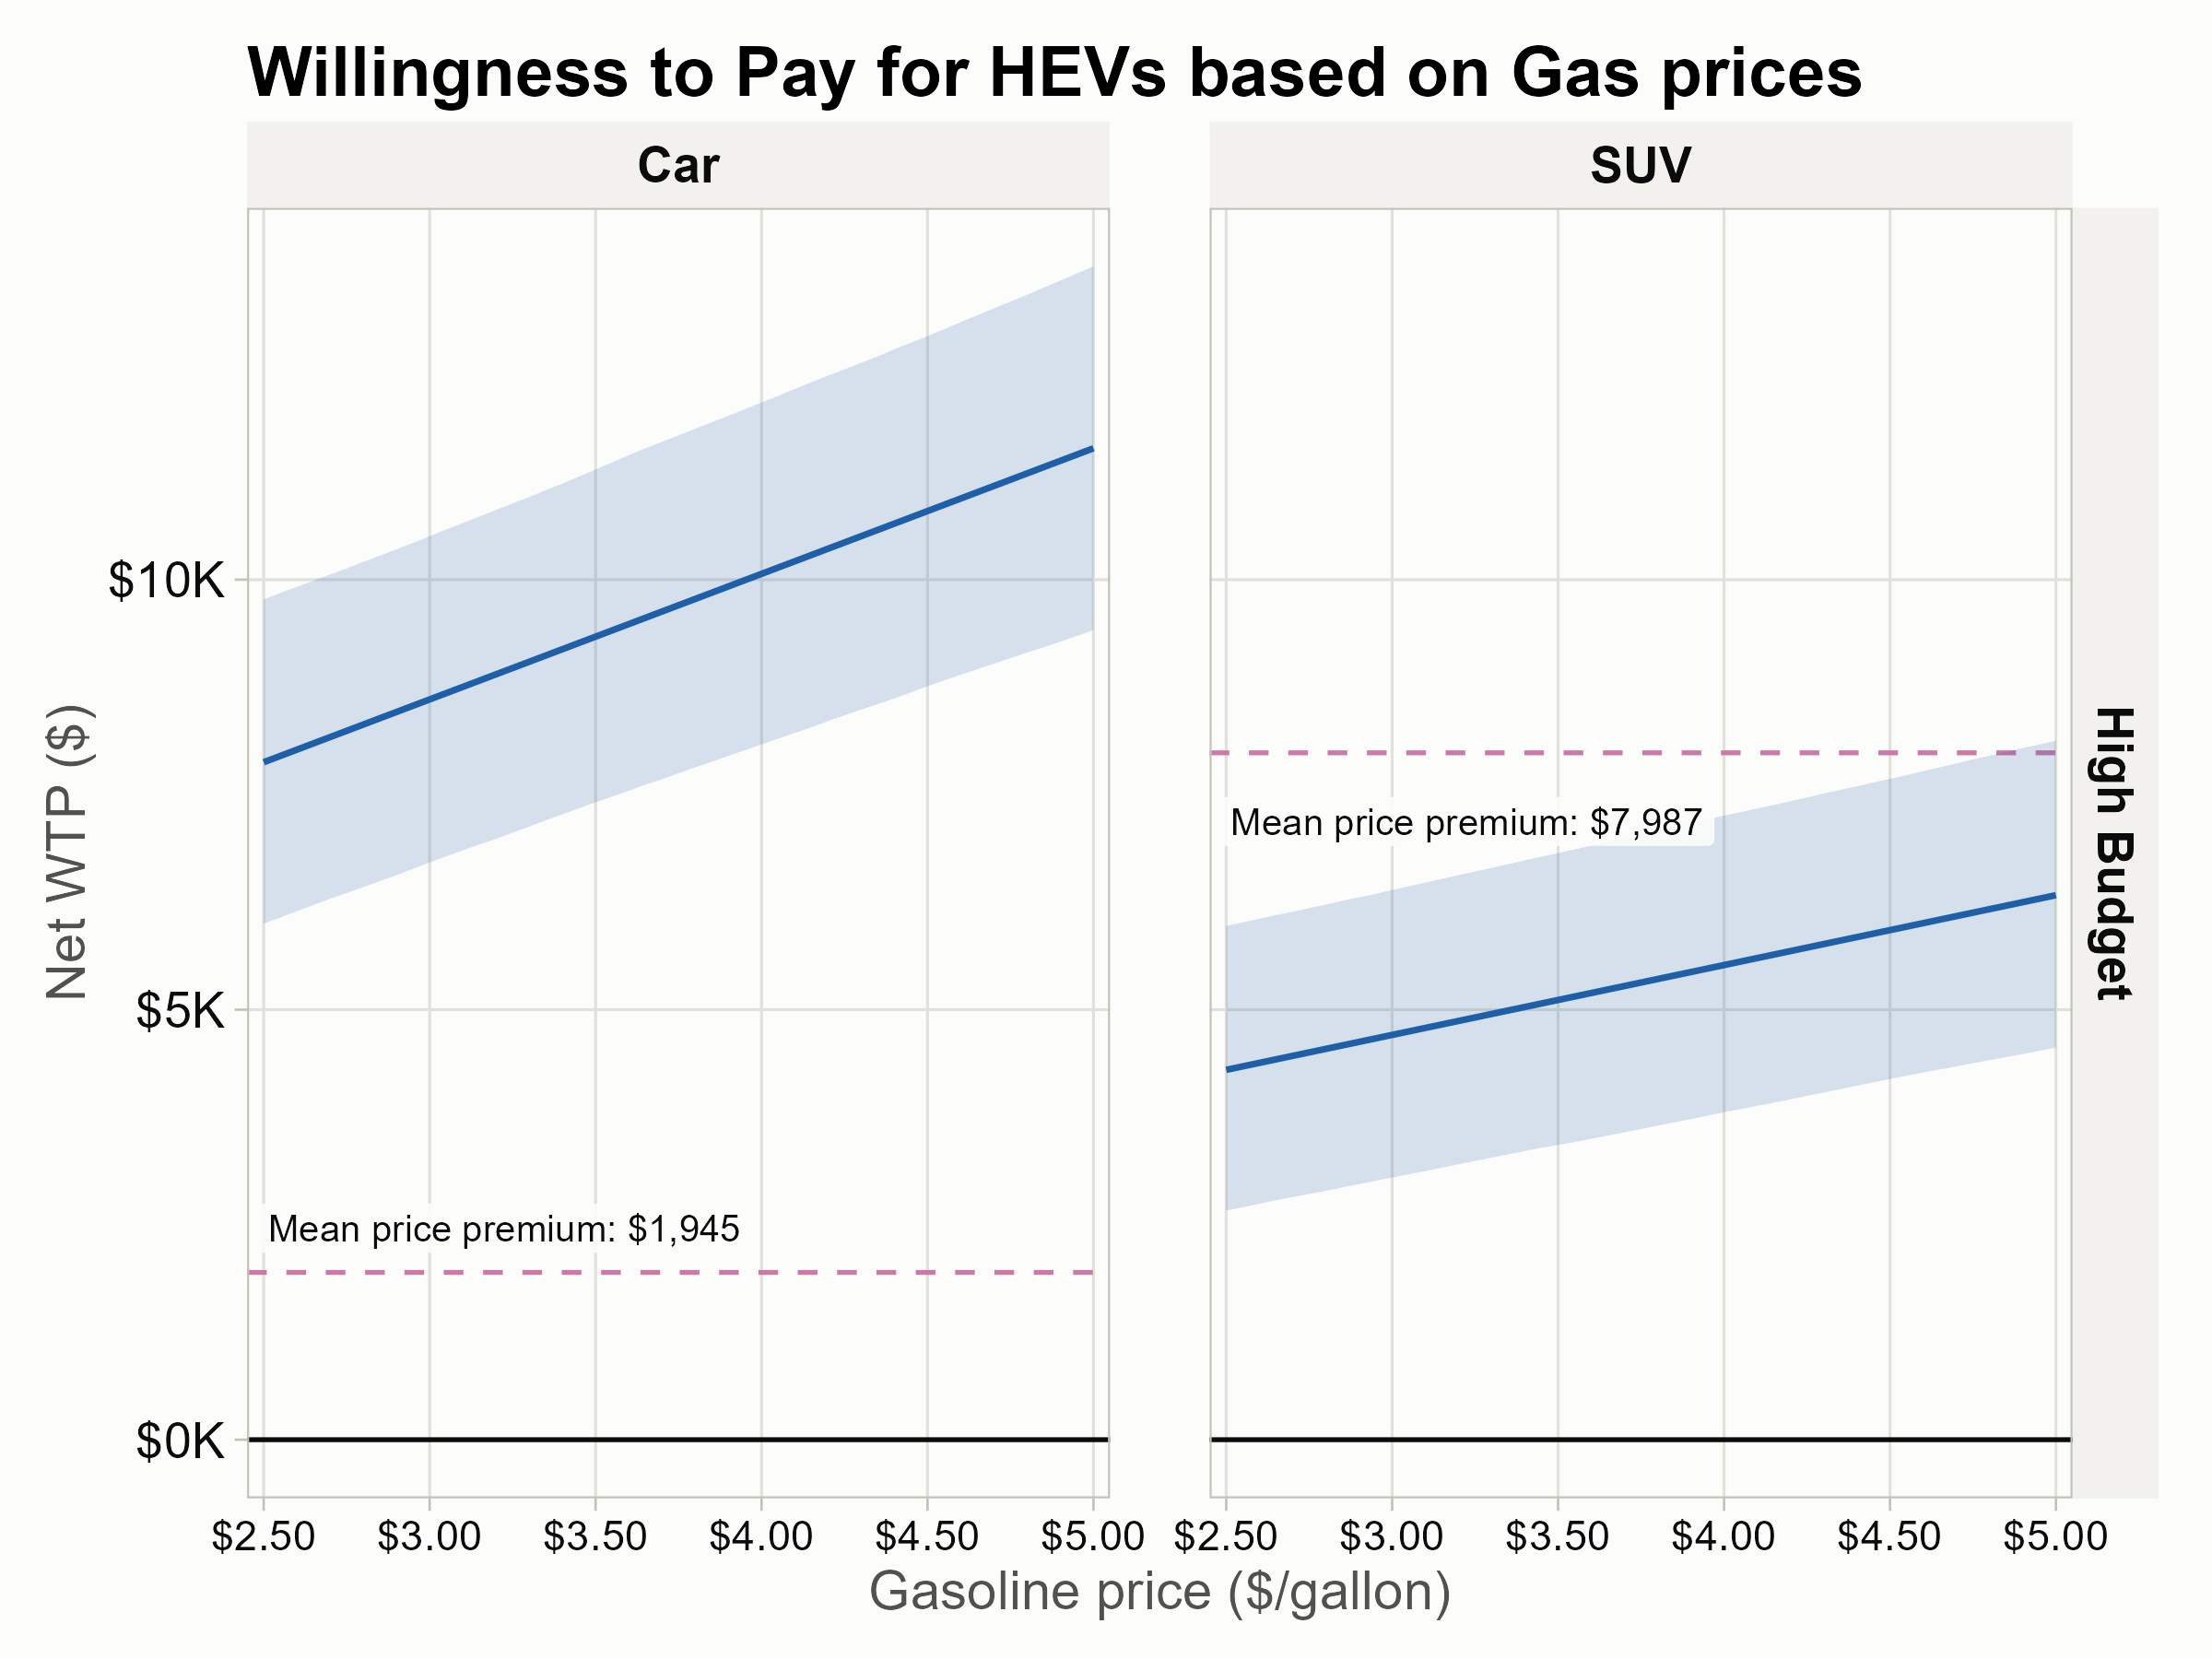
\includegraphics[width=0.85\textwidth]{images/vehicle_analysis/gas_price_sensitivity_hev.png}
    \caption{Net WTP versus gasoline price: HEV pairs. The blue line and band show simulated Net WTP (mean, 95\% interval) as the gasoline price varies from \$2.50 to \$5.00 per gallon; the dashed line is the observed mean real-market price premium at approximately three years of age. No matched HEV pair meeting the sample-size threshold was available in either low-budget segment.}
    \label{fig:gas_sensitivity_hev}
\end{figure}




\printcredits


\printbibliography


\end{document}
